% ============================================================
%  Prince Rupiya – H220536M – HIT 400 Project Document
%  Satellite-Based Tobacco Crop Health Monitoring System
%  Using Machine Learning and NDVI Analysis
%  Harare Institute of Technology, 2025
% ============================================================

\documentclass[12pt,a4paper]{report}

% ---- Page Layout ----
\usepackage[top=1in,bottom=1in,left=1.25in,right=1in,headheight=14pt]{geometry}

% ---- Fonts & Encoding ----
\usepackage[T1]{fontenc}
\usepackage[utf8]{inputenc}
\usepackage{mathptmx}          % Times New Roman

% ---- Line Spacing ----
\usepackage{setspace}
\onehalfspacing

% ---- Citations (Harvard / Author-Year) ----
\usepackage[round,authoryear,sort]{natbib}

% ---- Graphics ----
\usepackage{graphicx}
\usepackage{float}
\usepackage{caption}
\usepackage{subcaption}

% ---- TikZ for Diagrams ----
\usepackage{tikz}
\usetikzlibrary{shapes.geometric,shapes.misc,shapes.multipart,
                arrows.meta,positioning,fit,
                backgrounds,calc,decorations.pathreplacing}

% ---- Tables ----
\usepackage{booktabs}
\usepackage{array}
\usepackage{longtable}
\usepackage{tabularx}
\usepackage{multirow}
\usepackage{makecell}

% ---- Lists ----
\usepackage{enumitem}

% ---- Colours ----
\usepackage{xcolor}
\definecolor{hitblue}{RGB}{0,70,127}
\definecolor{lightgray}{RGB}{240,240,240}
\definecolor{darkgreen}{RGB}{0,128,0}
\definecolor{amber}{RGB}{255,191,0}
\definecolor{firebrick}{RGB}{178,34,34}

% ---- Maths ----
\usepackage{amsmath}
\usepackage{amssymb}

% ---- Code Listings ----
\usepackage{listings}
\lstset{basicstyle=\small\ttfamily,
        frame=single,
        backgroundcolor=\color{lightgray},
        breaklines=true}

% ---- Headers / Footers ----
\usepackage{fancyhdr}
\pagestyle{fancy}
\fancyhf{}
\fancyhead[L]{\small\leftmark}
\fancyhead[R]{\small Prince Rupiya | H220536M}
\fancyfoot[C]{\thepage}
\renewcommand{\headrulewidth}{0.4pt}

% ---- Hyperlinks ----
\usepackage{hyperref}
\hypersetup{colorlinks=true,
            linkcolor=hitblue,
            citecolor=hitblue,
            urlcolor=hitblue}

% ---- Chapter Titles ----
\usepackage{titlesec}
\titleformat{\chapter}[block]
  {\normalfont\Large\bfseries\color{hitblue}}
  {\chaptername\ \thechapter:}{0.5em}{}
\titlespacing*{\chapter}{0pt}{20pt}{15pt}

% ---- Table of Contents ----
\usepackage{tocloft}
\renewcommand{\cfttoctitlefont}{\Large\bfseries\color{hitblue}}
\renewcommand{\cftloftitlefont}{\Large\bfseries\color{hitblue}}
\renewcommand{\cftlottitlefont}{\Large\bfseries\color{hitblue}}

% ---- Gantt Chart ----
\usepackage{pgfgantt}

% ---- Verbatim ----
\usepackage{verbatim}

% ============================================================
%  Helper: diagram description box
% ============================================================
\usepackage{tcolorbox}
\tcbuselibrary{skins}
\newtcolorbox{diagrambox}[1]{
  colback=lightgray,colframe=hitblue,
  title={\textbf{Diagram Description — #1}},
  fonttitle=\small\bfseries,
  boxrule=0.8pt}

% ============================================================
\begin{document}
% ============================================================

% ---- Title Page ----
\begin{titlepage}
  \centering
  \vspace*{0.3cm}
  
\includegraphics[width=0.35\textwidth]{hit_logo.png}\\[0.5cm]
  {\large\bfseries HARARE INSTITUTE OF TECHNOLOGY}\\[0.2cm]
  {\large DEPARTMENT OF INFORMATION TECHNOLOGY}\\[0.2cm]
  {\large BTECH (HONS) INFORMATION TECHNOLOGY}\\[1.5cm]
  \rule{\linewidth}{0.5pt}\\[0.3cm]
  {\Large\bfseries Satellite-Based Tobacco Crop Health Monitoring\\
   System Using Machine Learning and NDVI Analysis}\\[0.3cm]
  \rule{\linewidth}{0.5pt}\\[1.2cm]
  {\large BY}\\[0.3cm]
  {\Large\bfseries PRINCE RUPIYA}\\[0.2cm]
  {\large H220536M}\\[1.2cm]
  {\large HIT 400}\\[0.8cm]
  {\large SUPERVISOR: MR P. MANYONGANISE}\\[1.5cm]
  \begin{minipage}{0.85\textwidth}\centering
    \normalsize
    This project report was submitted to the Harare Institute of
    Technology in partial fulfilment of the Bachelor of Technology
    (Hons) Degree in Information Technology.
  \end{minipage}\\[1.2cm]
  {\large 2025}
\end{titlepage}

% ---- Front Matter ----
\pagenumbering{roman}
\setcounter{page}{2}

% ---- Declaration ----
\chapter*{Declaration}
\addcontentsline{toc}{chapter}{Declaration}
\markboth{DECLARATION}{}

I, Prince Rupiya (H220536M), hereby declare that this project report is my own original work and has not been submitted, in whole or in part, for any other degree or qualification at Harare Institute of Technology or any other institution. Where the work of others has been used, it has been fully referenced and acknowledged in accordance with the Harvard referencing system.

\vspace{2cm}
\noindent\textbf{Student Signature:} \hrulefill \hspace{3cm} \textbf{Date:} \hrulefill

\vspace{1cm}
\noindent\textbf{Student Name:} Prince Rupiya \hspace{1cm} \textbf{Reg. Number:} H220536M

\vspace{2cm}
\noindent\textbf{Supervisor Signature:} \hrulefill \hspace{2.5cm} \textbf{Date:} \hrulefill

\vspace{1cm}
\noindent\textbf{Supervisor Name:} Mr P. Manyonganise \hspace{0.5cm} \textbf{Department:} Information Technology

% ---- Dedication ----
\chapter*{Dedication}
\addcontentsline{toc}{chapter}{Dedication}
\markboth{DEDICATION}{}

\begin{center}
\textit{To the smallholder tobacco farmers of Zimbabwe,\\
whose resilience and dedication to the land inspired this work.}

\vspace{1cm}
\textit{To my family, for their unwavering support and encouragement\\
throughout this academic journey.}

\vspace{1cm}
\textit{To the future of Zimbabwean agriculture — may technology\\
serve the hands that feed our nation.}
\end{center}

% ---- Acknowledgements ----
\chapter*{Acknowledgements}
\addcontentsline{toc}{chapter}{Acknowledgements}
\markboth{ACKNOWLEDGEMENTS}{}

I would like to express my sincere gratitude to Mr P. Manyonganise, my supervisor, whose expert guidance, patience, and constructive feedback shaped every aspect of this project. His deep knowledge of information systems and agricultural technology proved invaluable throughout the research and development process.

I am grateful to the Department of Information Technology at the Harare Institute of Technology for providing the academic foundation, resources, and environment that made this research possible.

I extend my appreciation to the open-source community behind Next.js, React-Leaflet, scikit-learn, Google Earth Engine, and the Open-Meteo project, whose freely available tools underpinned the technical implementation of this system.

I also thank my colleagues and fellow students who participated in system testing, provided feedback, and offered moral support throughout this endeavour.

Finally, I am deeply grateful to my family for their patience, encouragement, and sacrifices that sustained me through the demands of this programme.

% ---- Abstract ----
\chapter*{Abstract}
\addcontentsline{toc}{chapter}{Abstract}
\markboth{ABSTRACT}{}

Tobacco farming is a cornerstone of Zimbabwe's agricultural export economy, yet smallholder farmers continue to rely on manual, reactive monitoring methods that detect crop stress only after significant damage has occurred. This project presents the design and implementation of a satellite-based tobacco crop health monitoring system that integrates live Sentinel-2 multispectral imagery retrieved through the Google Earth Engine platform with machine learning and temporal trend analysis to deliver actionable, evidence-based insights to farmers through a web-based interface.

The system employs a logistic regression classifier trained on ground-truth satellite and weather observations to categorise crop health into three states: \emph{Healthy}, \emph{Moderate Stress}, and \emph{High Stress}, achieving 97\% classification accuracy. Feature engineering extracts five predictors from real satellite data: mean NDVI, NDVI trend slope, within-field NDVI variance, average temperature, and cumulative rainfall over a 14-to-30-day analysis window. Temporal trend analysis enables early detection of declining vegetation health before crops reach critical stress states, while within-field spatial variability analysis produces a heatmap overlay that identifies stress hotspots within user-drawn field polygons.

The web application is built on Next.js 14 with TypeScript, using React-Leaflet for interactive mapping and Prisma with PostgreSQL as the database backend. An explainable rule-based recommendation engine translates technical satellite data into plain-language farming advice covering irrigation scheduling, disease monitoring, and field inspection priorities.

The system contributes a cost-effective precision agriculture solution designed specifically for smallholder tobacco farmers in Zimbabwe, leveraging exclusively free and open data sources to eliminate subscription barriers. By combining live satellite imagery, machine learning inference, and transparent recommendation logic within a single accessible web platform, the system demonstrates that high-quality crop health monitoring can be achieved without expensive commercial infrastructure.

\vspace{0.5cm}
\noindent\textbf{Keywords:} crop health monitoring, machine learning, NDVI, precision agriculture,
satellite imagery, tobacco farming, Zimbabwe, Google Earth Engine, Sentinel-2, time-series analysis,
web application.

% ---- Tables of Contents / Figures / Tables ----
\tableofcontents
\listoffigures
\listoftables

% ---- List of Acronyms ----
\chapter*{List of Acronyms}
\addcontentsline{toc}{chapter}{List of Acronyms}
\markboth{LIST OF ACRONYMS}{}

\begin{longtable}{>{\bfseries}p{3cm} p{10cm}}
\toprule
Acronym & Definition \\
\midrule
API & Application Programming Interface \\
CRIM & Crop Remote Intelligence Monitor \\
DFD & Data Flow Diagram \\
ESA & European Space Agency \\
EVI & Enhanced Vegetation Index \\
FAO & Food and Agriculture Organization of the United Nations \\
GEE & Google Earth Engine \\
GIS & Geographic Information System \\
HTTP & Hypertext Transfer Protocol \\
HIT & Harare Institute of Technology \\
IT & Information Technology \\
JSON & JavaScript Object Notation \\
L2A & Level-2A (surface reflectance product of Sentinel-2) \\
ML & Machine Learning \\
NDVI & Normalized Difference Vegetation Index \\
NIR & Near-Infrared \\
ORM & Object-Relational Mapper \\
PostGIS & PostgreSQL Geographic Information System Extension \\
REST & Representational State Transfer \\
SQL & Structured Query Language \\
TIMB & Tobacco Industry and Marketing Board \\
UML & Unified Modelling Language \\
UI & User Interface \\
URL & Uniform Resource Locator \\
USD & United States Dollar \\
\bottomrule
\end{longtable}

% ============================================================
%  MAIN MATTER
% ============================================================
\cleardoublepage
\pagenumbering{arabic}
\setcounter{page}{1}

% ============================================================
\chapter{Introduction}
% ============================================================

\section{Introduction}

Agriculture remains the backbone of Zimbabwe's economy, accounting for approximately 12--15\% of gross domestic product and employing an estimated 60--70\% of the rural workforce \citep{moa2022}. Within this sector, tobacco stands as the country's most valuable cash crop. Zimbabwe is one of the world's largest tobacco producers, with the Tobacco Industry and Marketing Board recording auction sales exceeding 184 million kilogrammes in the 2022/2023 season, generating over USD 600 million in export revenue \citep{timb2023}. For smallholder farmers on communal and resettlement lands, tobacco cultivation provides a primary source of income, making the health of the crop a matter of direct economic survival.

Despite tobacco's strategic importance, the majority of smallholder farmers in Zimbabwe continue to rely on traditional monitoring methods rooted in manual observation and experience-based judgement \citep{nyoka2020}. Field inspections are time-consuming, subjective, and logistically constrained by terrain, distance, and seasonal weather. More critically, such methods detect crop stress—whether from water deficit, pest infestation, or nutrient deficiency—only after visible symptoms have appeared, by which point significant physiological damage has already occurred. The economic losses that follow are substantial: reduced leaf quality directly translates to lower grading at the auction floor and diminished farmer income \citep{rwizi2021}.

The advent of satellite remote sensing technology, machine learning, and open data infrastructure presents a transformative opportunity for Zimbabwean smallholder tobacco farming. The Normalized Difference Vegetation Index (NDVI), computed from multispectral satellite imagery, has been established as a reliable indicator of vegetation health for over four decades \citep{rouse1974}. Derived from the ratio of near-infrared to visible red reflectance, NDVI captures the physiological status of plant canopies with a sensitivity that predates visual symptom expression by several days. When integrated with weather data and machine learning classifiers, NDVI time-series can support early-warning systems that enable timely, targeted agricultural interventions.

This project proposes and implements a Satellite-Based Tobacco Crop Health Monitoring System that combines live Sentinel-2 multispectral imagery retrieved through the Google Earth Engine platform with logistic regression machine learning and temporal trend analysis, delivered through an accessible web-based interface. Farmers can define field boundaries through a polygon-drawing tool, trigger automated satellite analysis, and receive specific, explainable recommendations regarding irrigation, disease monitoring, and crop management. The system is designed exclusively around free and open data sources, eliminating the subscription barriers that have historically excluded smallholder farmers from precision agriculture tools.

This document covers Chapters 1 through 4 of the project report. Chapter 1 establishes the research context, motivation, problem statement, and objectives. Chapter 2 reviews related work, comparing existing precision agriculture platforms against the requirements identified for this system. Chapter 3 presents the requirements analysis, including feasibility assessment and work plan. Chapter 4 provides the system analysis, encompassing the existing system evaluation, the proposed solution, and formal system models.

\section{Motivation}

The motivation for this project derives from two converging realities observed in Zimbabwe's tobacco farming sector.

The first is economic. Tobacco contributes disproportionately to Zimbabwe's foreign currency earnings relative to other agricultural crops \citep{timb2023}. Yet yield variability among smallholder farmers remains high, driven in large part by late or missed detection of crop stress events. The Ministry of Lands, Agriculture, Fisheries, Water and Rural Development has identified precision farming as a strategic priority in the Zimbabwe Agricultural Development Strategy II 2021--2025, recognising that technology-enabled monitoring can significantly improve resource efficiency and yield stability \citep{moa2022}.

The second reality is technological. Satellite remote sensing data that once required specialised hardware and expensive processing infrastructure is now freely accessible through platforms such as Google Earth Engine \citep{gorelick2017}. The European Space Agency's Sentinel-2 satellites provide multispectral imagery at 10-metre spatial resolution on a 5-to-10-day revisit cycle, covering Zimbabwe with sufficient frequency to detect rapidly evolving crop stress events \citep{esa2023}. These data are publicly available at no cost, yet their utilisation by Zimbabwean farmers remains negligible due to the technical complexity of existing interfaces.

This project is motivated by the opportunity to bridge that gap: to translate freely available satellite data into accessible, actionable insights that smallholder tobacco farmers can use without specialised training or expensive equipment. A system that can detect declining NDVI trends in the 14 days before visible stress symptoms emerge gives farmers a meaningful window for intervention—one that the current manual inspection regime cannot provide.

\section{Problem Statement}

Current tobacco crop monitoring practices in Zimbabwe are characterised by significant limitations that undermine productivity and farmer income:

\begin{enumerate}
  \item \textbf{Reactive detection:} Crop stress events—including water deficit, pest infestation, and nutrient deficiency—are identified only after visible physical symptoms have developed, by which point yield loss is already inevitable \citep{nyoka2020}.

  \item \textbf{Temporal gaps:} Manual field inspections are episodic and infrequent, typically conducted weekly or fortnightly. Between inspections, stress conditions may develop, intensify, and cause irreversible damage without detection.

  \item \textbf{Spatial gaps:} Even when field visits occur, inspectors sample only parts of a field. Localised stress zones—a waterlogged corner, a section with compacted soil, or a pest entry point—are easily missed.

  \item \textbf{No integration of environmental data:} Monitoring decisions are rarely informed by systematic weather data. Rainfall, temperature, and drought indices that are highly predictive of stress events are not routinely incorporated into monitoring protocols.

  \item \textbf{Cost barriers to existing technology:} Commercial precision agriculture platforms that provide satellite-based crop monitoring charge subscription fees ranging from hundreds to thousands of USD per year, placing them far beyond the reach of smallholder farmers in Zimbabwe \citep{wolfert2017}.

  \item \textbf{Lack of localised solutions:} Few existing systems are calibrated for Zimbabwean growing conditions, tobacco-specific NDVI thresholds, or the realities of smallholder farming in Southern Africa \citep{rwizi2021}.
\end{enumerate}

There is therefore an urgent need for an integrated, accessible, and cost-effective system that uses satellite data and machine learning to monitor tobacco crop health in near-real time, detecting stress conditions before they manifest as visible damage and translating technical data into actionable farming decisions.

\section{Related Work}

Several platforms and research projects have explored the use of satellite data and precision agriculture technology, providing a foundation from which this system draws and against which it must be differentiated.

\subsection{Climate FieldView}

Climate FieldView, developed by The Climate Corporation—a subsidiary of Bayer AG—is one of the most widely deployed commercial precision agriculture platforms globally \citep{climcorp2023}. It provides satellite imagery, field-level analysis, yield mapping, and integration with farm machinery data. However, its commercial subscription model and design orientation towards large-scale North American farming operations make it inaccessible and contextually inappropriate for smallholder tobacco farmers in Zimbabwe. Its NDVI thresholds and recommendation logic are calibrated for maize, soybean, and other temperate grain crops rather than tropical cash crops such as tobacco.

\subsection{CropIn Technology}

CropIn Technology, based in India, offers a digital agriculture platform that has been deployed in parts of sub-Saharan Africa through NGO and government partnership programmes \citep{cropin2023}. The platform covers crop management, weather monitoring, and field analytics. While it demonstrates the feasibility of deploying digital agriculture tools in developing regions, CropIn's dependency on paid subscription tiers and its generic crop model—without tobacco-specific customisation—limit its applicability to Zimbabwe's smallholder sector. Furthermore, the system has not been validated against Zimbabwean field conditions or tobacco-specific NDVI behaviour.

\subsection{Taranis}

Taranis is an aerial intelligence platform that uses high-resolution drone and satellite imagery to detect crop diseases, pests, and nutrient deficiencies at a leaf level of precision \citep{taranis2023}. While technically sophisticated—achieving detection capabilities not possible with standard satellite imagery—Taranis is designed for large commercial farming operations and relies on drone hardware and per-hectare pricing that is economically prohibitive for smallholder farmers. Its strength lies in disease detection at a resolution this project does not attempt; its weakness is accessibility.

\subsection{Google Earth Engine and Open Research Tools}

The Google Earth Engine platform itself, along with open-source tools such as the Open Data Cube and Sen2Agri, provides freely accessible satellite data processing infrastructure that underpins an emerging body of agricultural remote sensing research \citep{gorelick2017}. Rwizi, Sibanda and Chimonyo \citep*{rwizi2021} demonstrate the application of GEE-based NDVI monitoring in Zimbabwean agricultural contexts, confirming the technical viability of the approach. However, these tools remain largely within the research domain, requiring programming expertise to use and offering no user-facing interface accessible to farmers.

\section{Hypothesis}

If Zimbabwean smallholder tobacco farmers are provided with a web-based system that combines live Sentinel-2 satellite NDVI data retrieved via Google Earth Engine with machine learning classification and temporal trend analysis, then they can receive early detection of crop stress conditions—specifically 7 to 14 days before visible symptoms develop—enabling timely interventions that reduce crop losses, improve resource allocation, and ultimately increase yield and income.

\section{Technical Objectives}

The main objective of this project is to design and implement a Satellite-Based Tobacco Crop Health Monitoring System that is accessible, accurate, and deployable by smallholder farmers in Zimbabwe. The specific objectives are:

\begin{enumerate}
  \item To design and implement a web-based platform that enables farmers to define field boundaries through interactive polygon drawing and trigger satellite-based crop health analysis on demand.

  \item To integrate live Sentinel-2 Level-2A multispectral imagery through the Google Earth Engine API to compute real NDVI values for user-defined field polygons, replacing estimated data with actual satellite measurements.

  \item To develop and train a logistic regression machine learning classifier on ground-truth satellite and weather observations to classify tobacco crop health into three categories: \emph{Healthy}, \emph{Moderate Stress}, and \emph{High Stress}.

  \item To implement temporal NDVI trend analysis over a 14-to-30-day observation window using linear regression, enabling early detection of declining vegetation health trajectories before crops reach critical stress states.

  \item To provide within-field spatial variability analysis using per-pixel Sentinel-2 NDVI distributions, generating a heatmap overlay that identifies and localises stress hotspots within drawn field polygons.

  \item To design an explainable rule-based recommendation system that translates technical satellite data and model predictions into plain-language farming advice covering irrigation, disease monitoring, and field inspection.

  \item To deploy the system using a scalable architecture that separates Python-based machine learning model training from JavaScript-based inference, enabling serverless deployment without requiring Python runtime infrastructure.
\end{enumerate}

\section{Expected Results}

The successful implementation of this system is expected to yield the following outcomes:

\begin{itemize}
  \item A fully functional web application accessible via standard web browsers, requiring no software installation, enabling Zimbabwean tobacco farmers to monitor crop health using live satellite data.

  \item A logistic regression crop health classifier achieving accuracy exceeding 90\% on held-out ground-truth test data, with balanced precision and recall across all three health categories.

  \item Temporal trend detection capability that identifies declining NDVI trajectories within a 14-to-30-day analysis window, issuing early-warning alerts before crops reach the High Stress threshold.

  \item Within-field heatmap visualisation that highlights specific areas of localised stress within farmer-defined field polygons, enabling targeted rather than uniform interventions.

  \item A recommendation engine that provides specific, evidence-linked advice for irrigation scheduling, disease risk monitoring, and agronomist inspection, with each recommendation accompanied by the data observations that triggered it.

  \item A zero-cost data architecture that relies exclusively on the Google Earth Engine free research tier and the Open-Meteo open weather API, eliminating recurring subscription costs for deployment and operation.

  \item Improved farmer decision-making capability, with the expectation that early stress detection will reduce crop losses from water stress and disease by enabling interventions within the effective treatment window.
\end{itemize}

\section{Ethics Considerations}

\begin{itemize}
  \item \textbf{Data Privacy and Consent:} The system collects farmer names, email addresses, and geographic field location data. All personal data is stored in a PostgreSQL database secured with role-based access controls and encrypted passwords using bcrypt hashing. Farmers retain full ownership of their field data, and no data is shared with third parties without explicit consent. The system complies with data protection principles outlined in Zimbabwe's Cybersecurity and Data Protection Act (2021).

  \item \textbf{Data Accuracy and Transparency:} NDVI values are derived from real Sentinel-2 multispectral imagery and are accompanied by the observation date, cloud cover status, and analysis window parameters, allowing users to assess data quality. The system explicitly communicates uncertainty where cloud cover reduces the number of usable satellite observations. Each recommendation is linked to the specific data observation that triggered it, ensuring farmers can evaluate and, if necessary, override system advice.

  \item \textbf{Algorithmic Fairness:} The machine learning model is trained on ground-truth data that reflects the natural variation in Zimbabwean tobacco field conditions. Model performance is evaluated separately across all three health categories to detect and mitigate class-specific bias. Thresholds are reviewed against agronomic literature to ensure they reflect biologically meaningful boundaries rather than artefacts of the training data.

  \item \textbf{Accessibility and Inclusivity:} The web interface is designed for use with basic internet connectivity and entry-level smartphones. Text is presented in plain English at a reading level appropriate for users with secondary school education. The system does not assume technical literacy beyond the ability to navigate a standard website.

  \item \textbf{Environmental Responsibility:} The system promotes precision application of irrigation water and agrochemicals, directly supporting reduced resource waste and environmental impact. By enabling targeted interventions in specific stress zones rather than uniform field-wide treatment, the system actively encourages sustainable farming practices.

  \item \textbf{Satellite Data Use:} All satellite imagery is accessed through the Google Earth Engine platform under its terms of service for research and non-commercial use. Sentinel-2 imagery is provided freely by the European Space Agency under the Copernicus Open Access Data Policy and carries no use restrictions.
\end{itemize}

\section{Conclusion}

This chapter has established the context, motivation, and objectives of the Satellite-Based Tobacco Crop Health Monitoring System. The challenges facing Zimbabwean smallholder tobacco farmers—reactive detection, temporal and spatial monitoring gaps, and cost barriers to existing technology—are well-documented and directly addressable through the combination of freely available Sentinel-2 satellite imagery, machine learning classification, and a user-centred web interface.

The system proposed here is not merely a research prototype. It is designed for real deployment, using free and open data sources, a scalable technology stack, and an explainable recommendation engine that respects the knowledge and agency of the farmers it serves. The chapters that follow build from this foundation: reviewing the existing landscape of precision agriculture systems, defining the requirements that must be met, and presenting the system analysis that will guide implementation.

% ============================================================
\chapter{Literature Review}
% ============================================================

\section{Introduction}

Precision agriculture platforms have evolved substantially since the early NDVI-based vegetation monitoring systems of the 1970s. What began as research-grade tools requiring specialised remote sensing expertise have matured into integrated platforms combining satellite imagery, weather data, field sensors, and machine learning within commercially deployed systems \citep{wolfert2017}. For this project to situate its contribution clearly, it is necessary to evaluate the current landscape of relevant systems against the specific requirements of smallholder tobacco farming in Zimbabwe.

This chapter reviews five platforms and systems that represent the contemporary state of satellite-based and digital precision agriculture: FarmLogs, SatAgro, Farmerline, Digital Green, and Regrow Ag. Each is assessed for its technical capabilities, accessibility, and suitability for the Zimbabwean smallholder tobacco context. The chapter concludes by identifying the systemic gaps that justify the system proposed in this project.

The broader academic literature on NDVI-based crop monitoring, machine learning for agriculture, and decision support systems is reviewed, establishing the theoretical foundations on which this project's methodology is built.

\section{Related Works}

\subsection{FarmLogs (TELUS Agriculture)}

FarmLogs, subsequently acquired by TELUS Agriculture, is a cloud-based farm management platform that provides satellite field imagery, crop health monitoring through NDVI visualisation, and weather-based planting recommendations \citep{farmerline2023}. The platform is designed primarily for North American grain farming operations, offering integration with GPS-tracked field equipment, soil sampling data, and yield history. Its NDVI imagery is derived from Landsat and Sentinel-2 satellite data, processed and presented as a time-series health index.

From the perspective of this project's requirements, FarmLogs demonstrates the technical viability of web-based NDVI crop monitoring. However, it operates on a subscription pricing model that has historically ranged from USD 300 to USD 600 per year for its full feature set \citep{wolfert2017}. This cost structure is economically prohibitive for Zimbabwean smallholder tobacco farmers whose net annual income from a single season may be comparable to or lower than the subscription fee. Furthermore, FarmLogs provides no tobacco-specific thresholds, no temporal trend alerting calibrated to tropical growing seasons, and no spatial hotspot detection within field polygons beyond basic imagery overlays. As \citet{liakos2018} observe, effective agricultural decision support systems must incorporate domain-specific agronomic knowledge to be operationally useful, a criterion FarmLogs does not meet for tobacco cultivation.

\subsection{SatAgro}

SatAgro is a European satellite monitoring service built on Sentinel-1 and Sentinel-2 imagery, providing NDVI time-series, field zoning, and variable-rate application zone maps for European cereal and oilseed farming \citep{satagtro2023}. The platform demonstrates a technically sophisticated use of multispectral satellite data: it computes NDVI statistics per field polygon, generates within-field variability maps, and supports precision application of fertilisers through variable-rate prescription maps.

SatAgro's within-field variability analysis is the closest existing commercial analogue to the spatial hotspot functionality implemented in this project. However, SatAgro is operationally restricted to European markets and calibrated for temperate-climate crops. It has no deployment in Africa and no provision for tropical growing conditions, cloud-season imagery gaps typical of Zimbabwe's rainy season from November to March, or tobacco-specific agronomic thresholds. Technically, SatAgro also requires a subscription and does not expose its satellite processing pipeline for free access. The comparison nonetheless validates the within-field variability approach as a technically proven capability worth implementing in the Zimbabwean context.

\subsection{Farmerline}

Farmerline is a Ghanaian agri-tech company that has deployed digital farming tools across several West and East African markets, providing weather forecasts, crop management advice, and market price information through both smartphone applications and interactive voice response systems for feature phones \citep{farmerline2023}. Its design specifically targets smallholder farmers in developing regions with limited internet connectivity and technical literacy, making it contextually closer to this project's deployment environment than the commercial platforms reviewed above.

Farmerline demonstrates that agricultural technology can be adapted successfully for smallholder farmer contexts in sub-Saharan Africa. However, the platform does not incorporate satellite imagery or NDVI-based crop health analysis. Its agricultural advice is rule-based and generic, derived from crop calendars and generalised weather data rather than field-specific satellite observations. As \citet{rose2016} argue, decision support systems that rely on generic rules without field-level observational data cannot provide the specificity needed to guide individual farm management decisions effectively. Farmerline's success in user adoption nonetheless validates the user-interface design principles — plain language, minimal technical terminology, and accessibility on entry-level hardware — that this project adopts.

\subsection{Digital Green}

Digital Green is an international NGO-driven platform that uses video-based peer learning and digital tools to improve smallholder farmer practice across South Asia and Sub-Saharan Africa, including Zimbabwe \citep{digitalgreen2023}. The platform has worked with Zimbabwe's Ministry of Agriculture to disseminate good agricultural practices through community video screenings and mobile-based advisory services. Digital Green's programmes have demonstrated measurable yield improvements in smallholder farming communities, validating the effectiveness of technology-mediated agricultural extension in the Zimbabwean context.

Digital Green does not, however, provide satellite monitoring, NDVI analysis, or field-level crop health assessment. Its contribution is in the dissemination of general best practices rather than in field-specific precision monitoring. This distinction is important: the system proposed in this project aims to complement extension services like Digital Green by providing the field-level observational data that extension advice cannot replace. The two approaches are complementary rather than competing.

\subsection{Regrow Ag}

Regrow Ag is a precision agriculture platform focused on sustainable crop production measurement and carbon sequestration quantification, using satellite data, crop simulation models, and machine learning to produce field-level sustainability metrics for large agricultural supply chains \citep{regrow2023}. While technically advanced, Regrow Ag is designed for use by agricultural commodity companies and large cooperatives rather than individual smallholder farmers. Its satellite analysis pipeline processes Sentinel-2 and Landsat imagery at scale, but the results are presented through corporate sustainability dashboards rather than farmer-facing interfaces.

Regrow Ag is the only platform reviewed here that explicitly incorporates temporal NDVI trend analysis within its methodology, computing seasonal vegetation trajectories to estimate crop productivity and carbon fluxes. This validates the temporal trend analysis approach at the core of this project. However, Regrow Ag's inaccessibility to individual farmers and its focus on carbon markets rather than crop health monitoring leave a clear gap in the precision agriculture landscape for a farmer-facing temporal monitoring system.

\subsection{Academic Foundations}

Beyond commercial platforms, this project draws on a well-established academic literature in satellite remote sensing, machine learning for agriculture, and decision support systems.

\citet{rouse1974} established NDVI as a fundamental metric for vegetation health monitoring, demonstrating its correlation with biomass and photosynthetic activity. Subsequent work by \citet{tucker1979} confirmed NDVI's sensitivity to vegetation stress through its relationship with chlorophyll absorption in the red band and structural scattering in the near-infrared, establishing the physiological basis for NDVI as an early-warning indicator that predates visual symptom expression.

\citet{weiss2020} provide a comprehensive meta-review of remote sensing applications in agriculture, demonstrating across 110 studies that satellite-derived vegetation indices achieve reliable classification of crop health status with prediction accuracy exceeding 80\% in most controlled studies. Sentinel-2 imagery, with its 10-metre spatial resolution and 5-to-10-day revisit frequency, is identified as the most suitable freely available satellite data source for field-scale crop monitoring.

In the domain of machine learning for agriculture, \citet{liakos2018} review 40 studies and identify logistic regression, support vector machines, and random forests as the most widely applied classification algorithms, noting that logistic regression—despite its simplicity—frequently achieves accuracy comparable to more complex models on datasets where features are well-engineered and class boundaries are relatively stable. This observation directly motivates the algorithm selection in this project. \citet{chlingaryan2018} further demonstrate that the combination of NDVI with weather variables (temperature and precipitation) consistently improves crop health classification accuracy over NDVI-only models.

The importance of explainability in agricultural decision support systems is emphasised by \citet{rose2016}, who find through a systematic review of 40 agricultural decision tools that farmer adoption rates are strongly correlated with system transparency: tools that explain the reasoning behind recommendations are significantly more likely to be trusted and acted upon than those that provide recommendations without justification. This finding is central to the design of this project's recommendation engine.

Finally, \citet{wolfert2017} review the architecture of big data systems in precision agriculture, noting the importance of modular, scalable architectures that separate data acquisition, analysis, and presentation layers—a design principle directly implemented in this project's three-layer architecture.

\section{Conclusion}

The review of existing platforms reveals a consistent pattern across the commercial landscape: the systems with the strongest technical capabilities—FarmLogs, SatAgro, Regrow Ag—are designed for large-scale operations in developed-market geographies and require subscription fees that exclude smallholder farmers. The systems that have successfully reached smallholder farmers in developing regions—Farmerline, Digital Green—lack satellite-based crop health monitoring and field-level precision. No existing platform combines live satellite NDVI analysis, temporal trend detection, within-field spatial variability mapping, and tobacco-specific recommendation logic in a freely accessible, farmer-facing web interface designed for Zimbabwean conditions.

The academic literature confirms the technical validity of the approach: NDVI derived from Sentinel-2 imagery is a reliable, early-warning indicator of crop stress; logistic regression trained on NDVI and weather features achieves high classification accuracy; and explainable recommendation systems achieve higher farmer adoption than black-box alternatives. Temporal trend analysis over multi-week observation windows is identified as a particularly valuable but underutilised capability in farmer-facing tools.

These findings collectively justify the system proposed in this project and define the specific technical and design requirements addressed in the chapters that follow.

% ============================================================
\chapter{Requirements Analysis}
% ============================================================

\section{Introduction}

Requirements engineering is the process of systematically identifying, documenting, and validating the needs that a system must satisfy before design and development begin. \citet{sommerville2016} argues that errors introduced at the requirements stage are consistently the most expensive to correct, as each subsequent development phase amplifies the cost of addressing a misunderstood or missing requirement. For this project, requirements were elicited through a combination of direct observation of current tobacco farming monitoring practices, structured interviews with farmers and agricultural extension officers, a distributed questionnaire, document analysis of existing systems and research literature, and prototyping exercises conducted with prospective users.

This chapter first evaluates alternative development approaches, then defines user requirements, assesses system feasibility across technical, economic, and operational dimensions, and concludes with a work plan for the project.

\subsection{Evaluate Alternatives}

Before committing to a custom-built system, two principal alternatives were systematically evaluated.

The first alternative was to deploy and configure an existing commercial precision agriculture platform for use by Zimbabwean tobacco farmers. Platforms reviewed in Chapter 2, including FarmLogs and SatAgro, were assessed against the specific requirements of smallholder tobacco monitoring in Zimbabwe. This alternative was rejected for three reasons: prohibitive subscription costs that cannot be sustained by smallholder farmers; absence of tobacco-specific NDVI thresholds and recommendation logic; and lack of deployment or support infrastructure in Zimbabwe. As \citet{wolfert2017} observe, commercial precision agriculture platforms designed for developed-market farming contexts frequently fail in technology transfer to smallholder environments due to structural mismatches in cost, connectivity, and agronomic calibration.

The second alternative was to develop a plugin or extension layer on top of an existing open-source GIS platform such as QGIS or Open Data Cube. While this would leverage existing satellite data processing infrastructure, it would require users to install and configure specialised GIS software—a technical barrier that is inconsistent with the accessibility requirements for smallholder farmers with basic digital literacy. Additionally, these platforms provide no machine learning inference, no recommendation engine, and no web-based user interface deployable without local installation.

The custom development approach was therefore selected as the most appropriate path, allowing the system to be designed specifically around the requirements of Zimbabwean tobacco farmers without inheriting the constraints of existing platforms.

\subsection{Outsourcing}

Outsourcing the development to a commercial software house or freelance developer was considered and rejected. The system's requirement for tobacco-specific agronomic knowledge, intimate familiarity with the Google Earth Engine API for Zimbabwean satellite data, and iterative design refinement based on farmer feedback makes close in-house control of the development process essential. \citet{pfleeger2010} note that outsourcing is most effective when requirements are fully specified and stable before development begins—conditions that do not hold in a research and prototyping context where requirements evolve through building, testing, and farmer feedback. Maintaining full control of the codebase is also necessary for the long-term academic contribution and potential open-source release of the system.

\subsection{Improvement Over the Current System}

The proposed system improves on the existing manual monitoring approach in the following concrete ways:

\begin{itemize}
  \item \textbf{Timeliness:} Satellite analysis is available every 5--10 days, aligned with Sentinel-2 revisit cycles, compared to the weekly or fortnightly manual field inspections that characterise current practice.
  \item \textbf{Objectivity:} NDVI values derived from satellite multispectral reflectance are quantitative and reproducible, replacing subjective visual assessments by individual inspectors.
  \item \textbf{Early detection:} Temporal trend analysis detects declining NDVI trajectories 7--14 days before visible stress symptoms develop, enabling intervention within the effective treatment window.
  \item \textbf{Spatial precision:} Within-field heatmap analysis identifies localised stress zones that aggregate inspection would miss.
  \item \textbf{Cost:} The system eliminates the cost of frequent manual field inspections and uses exclusively free data sources, reducing the monitoring cost per hectare substantially.
\end{itemize}

\citet{pfleeger2010} argue that usability improvements that directly affect the timeliness and accuracy of decisions are not cosmetic enhancements but core system requirements; this principle underpins the design priorities throughout this project.

\subsection{Development Approach}

The system is developed using a modular, three-layer architecture that separates data acquisition, machine learning analysis, and user interface concerns. This separation enables independent development, testing, and updating of each layer without requiring changes to others. The machine learning model is trained offline in Python using scikit-learn and exported as a JSON weight file for consumption by the JavaScript web application, enabling serverless deployment without Python runtime infrastructure \citep{pedregosa2011}. The web application is built on Next.js 14 with the App Router architecture, TypeScript for type safety, and Prisma as the database ORM. An Agile development methodology is applied, with two-week sprints, iterative prototyping, and weekly supervisor reviews.

\section{User Requirements}

Three distinct user roles interact with the system, each with specific requirements:

\noindent\textbf{Farmer Requirements:}
\begin{itemize}[leftmargin=2cm]
  \item The system shall allow farmers to register and log in using email and password credentials.
  \item The system shall enable farmers to define field boundaries by drawing polygons on an interactive satellite map.
  \item The system shall allow farmers to trigger a crop health analysis for any defined field with a single action.
  \item The system shall present analysis results in plain language with colour-coded health status indicators.
  \item The system shall provide specific, actionable recommendations for irrigation, disease monitoring, and field inspection.
  \item The system shall display a historical list of previous analyses for each field.
  \item The system shall function on standard web browsers on smartphones with mobile data connectivity.
\end{itemize}

\noindent\textbf{Agronomist Requirements:}
\begin{itemize}[leftmargin=2cm]
  \item The system shall allow agronomists to view satellite analysis results for fields assigned to them.
  \item The system shall present NDVI time-series trend data in chart form to support agronomist assessment.
  \item The system shall provide within-field heatmap visualisation of NDVI spatial variability.
  \item The system shall display the raw feature values (mean NDVI, trend slope, variance, temperature, rainfall) underlying each classification decision.
  \item The system shall allow agronomists to access analysis history across multiple growing seasons.
\end{itemize}

\noindent\textbf{System Administrator Requirements:}
\begin{itemize}[leftmargin=2cm]
  \item The system shall allow administrators to manage user accounts, including creation, role assignment, and deactivation.
  \item The system shall allow administrators to configure system-level parameters including NDVI threshold values and recommendation rule weights.
  \item The system shall provide administrators with system usage logs for auditing and monitoring.
  \item The system shall enforce secure authentication and role-based access controls for all administrative functions.
\end{itemize}

\subsection{Data Collection Phase}

Requirements were elicited through the following methods, following the structured elicitation framework recommended by \citet{sommerville2016}:

\noindent\textbf{Structured Interviews:} Semi-structured interviews were conducted with five tobacco farmers in the Mvurwi farming area of Mashonaland Central Province and three agricultural extension officers from the Agritex provincial office. The interviews explored current monitoring practices, frequency of field inspections, awareness of satellite technology, and willingness to adopt a digital monitoring system. Key findings included: all five farmers reported detecting water stress only after wilting was visible; none were aware of NDVI as a monitoring technique; all expressed strong interest in a system that could provide advance warning of stress conditions.

\noindent\textbf{Questionnaire:} A structured questionnaire was distributed to 20 IT and agriculture stakeholders including smallholder farmers, cooperative managers, and extension officers. The questionnaire is presented below.

\vspace{0.5cm}
\noindent\rule{\linewidth}{0.4pt}
\vspace{0.1cm}

\noindent\textbf{Sample Questionnaire: Tobacco Crop Monitoring Needs Assessment}

\vspace{0.2cm}
\noindent\textit{Purpose: This questionnaire gathers information on current crop monitoring practices and technology readiness among tobacco farming stakeholders in Zimbabwe, in support of the development of a Satellite-Based Tobacco Crop Health Monitoring System. All responses are used for academic and system development purposes only.}

\vspace{0.3cm}
\noindent\textbf{Section A: Respondent Information}

\begin{enumerate}
  \item What is your role?\\
  $\square$ Smallholder Tobacco Farmer \quad $\square$ Large-Scale Farmer \quad $\square$ Agronomist \quad $\square$ Extension Officer \quad $\square$ Other: \underline{\hspace{3cm}}

  \item How many hectares of tobacco do you grow per season?\\
  $\square$ Less than 2 ha \quad $\square$ 2--5 ha \quad $\square$ 5--10 ha \quad $\square$ More than 10 ha

  \item How many years of farming experience do you have?\\
  $\square$ Less than 3 years \quad $\square$ 3--7 years \quad $\square$ 7--15 years \quad $\square$ More than 15 years
\end{enumerate}

\noindent\textbf{Section B: Current Monitoring Practices}

\begin{enumerate}[resume]
  \item How do you currently monitor your tobacco crop health?\\
  $\square$ Visual inspection \quad $\square$ Agronomist visits \quad $\square$ Sensor/equipment \quad $\square$ No systematic monitoring

  \item How frequently do you inspect your fields?\\
  $\square$ Daily \quad $\square$ Every 2--3 days \quad $\square$ Weekly \quad $\square$ Fortnightly \quad $\square$ Monthly

  \item When are stress conditions (water stress, disease) typically detected?\\
  $\square$ Before any visible symptoms \quad $\square$ When early symptoms appear \quad $\square$ After significant damage is visible \quad $\square$ After crop loss has occurred
\end{enumerate}

\noindent\textbf{Section C: Technology Readiness}

\begin{enumerate}[resume]
  \item Do you own or have access to a smartphone?\\
  $\square$ Yes, with reliable internet \quad $\square$ Yes, with limited internet \quad $\square$ No, feature phone only \quad $\square$ No mobile phone

  \item Are you aware of satellite-based crop monitoring tools?\\
  $\square$ Yes, and I use them \quad $\square$ Yes, but I do not use them \quad $\square$ I have heard of them \quad $\square$ No

  \item Would you use a free web-based tool that shows your field's crop health from satellite data?\\
  $\square$ Strongly agree \quad $\square$ Agree \quad $\square$ Neutral \quad $\square$ Disagree \quad $\square$ Strongly disagree
\end{enumerate}

\noindent\textbf{Section D: Decision Support Needs}

\begin{enumerate}[resume]
  \item What information would be most valuable in a crop monitoring system? (Select all that apply)\\
  $\square$ Water stress level \quad $\square$ Disease risk alert \quad $\square$ Irrigation schedule \quad $\square$ Yield prediction \quad $\square$ Field health trend over time \quad $\square$ Specific affected zones within the field

  \item How important is it to receive farming advice linked to your specific field's satellite data?\\
  $\square$ Very important \quad $\square$ Important \quad $\square$ Moderately important \quad $\square$ Not important

  \item What is the biggest challenge in your current monitoring approach?\\
  $\square$ Missing stress until too late \quad $\square$ Cost of field inspections \quad $\square$ Labour availability \quad $\square$ Inaccurate assessments \quad $\square$ Other: \underline{\hspace{3cm}}
\end{enumerate}

\noindent\textit{Thank you for your participation. Your responses directly inform the design of an accessible, farmer-focused satellite monitoring system for Zimbabwean tobacco farming.}

\vspace{0.1cm}
\noindent\rule{\linewidth}{0.4pt}
\vspace{0.3cm}

\noindent\textbf{Document Analysis:} Existing Agritex crop assessment forms, the TIMB annual report \citep{timb2023}, and the Ministry of Agriculture's Zimbabwe Agricultural Development Strategy II \citep{moa2022} were reviewed to identify which crop health parameters are currently collected and at what frequency, informing the design of the analysis output format.

\noindent\textbf{Direct Observation:} Observation of a tobacco field inspection session in Mvurwi district confirmed that inspectors assess only three to five points within a field during a standard visit, missing an estimated 60--80\% of field area. This observation directly motivated the within-field spatial variability analysis requirement.

\subsection{Technical Feasibility}

The proposed system relies on well-established, extensively documented technologies. The Google Earth Engine API for Sentinel-2 data retrieval is a mature service with comprehensive documentation and an active developer community, and has been used in peer-reviewed agricultural monitoring research in Zimbabwe \citep{rwizi2021}. The Next.js, React, and scikit-learn frameworks are among the most widely used web and machine learning libraries respectively, with large communities, long-term support commitments, and extensive learning resources. All chosen technologies are within the developer's existing skill set, and no significant technical risks that would prevent delivery within the project timeline have been identified. \citet{perera2015} highlight that systems built on open, well-supported APIs with clear documentation have substantially lower technical risk profiles than those dependent on proprietary or experimental interfaces.

\subsection{Hardware Requirements}

\begin{itemize}
  \item \textbf{Development machine:} Intel Core i-series or equivalent processor, minimum 8~GB RAM (16~GB recommended), 256~GB SSD storage minimum, running Windows 10/11, macOS, or Ubuntu Linux.
  \item \textbf{Server / cloud:} Vercel or Netlify platform for Next.js deployment (free tier available); managed PostgreSQL service (e.g., Neon, Supabase free tier) for database hosting.
  \item \textbf{End-user device:} Any smartphone or computer with a modern web browser (Chrome, Firefox, Safari) and mobile data or Wi-Fi connectivity.
\end{itemize}

\subsection{Software Requirements}

\begin{itemize}
  \item \textbf{Operating System:} Windows 11 / macOS 14 / Ubuntu 22.04 LTS
  \item \textbf{Runtime Environments:} Node.js 20 LTS, Python 3.11
  \item \textbf{Web Framework:} Next.js 14 (App Router)
  \item \textbf{Frontend:} React 18, TypeScript 5, React-Leaflet 4, Leaflet.draw
  \item \textbf{Database:} PostgreSQL 16 with PostGIS 3.4 extension
  \item \textbf{ORM:} Prisma 5
  \item \textbf{Machine Learning:} scikit-learn 1.3, pandas 2, matplotlib 3.7
  \item \textbf{Satellite API:} Google Earth Engine Python API (earthengine-api)
  \item \textbf{Weather API:} Open-Meteo (free, no authentication required)
  \item \textbf{Development Environment:} Visual Studio Code
  \item \textbf{Version Control:} Git with GitHub
  \item \textbf{Containerisation:} Docker (optional, for local PostgreSQL development)
\end{itemize}

\subsection{Technical Expertise}

Successful development requires proficiency in the following areas: TypeScript and React for frontend development; Next.js App Router and REST API design for backend development; Python and scikit-learn for machine learning model training and evaluation; PostgreSQL and PostGIS for spatial data management; the Google Earth Engine API for satellite data retrieval and NDVI computation; Git for version control and collaborative development; and basic information security practices including authentication, password hashing, and HTTPS enforcement.

\section{Economic Feasibility}

The project is economically justified on the basis of both its development costs and its expected operational benefits to Zimbabwean tobacco farmers.

\subsection{Cost-Benefit Analysis}

Table~\ref{tab:costbenefit} presents a two-year financial projection for the system's development and operational costs against anticipated savings and income improvements for a representative cohort of 50 smallholder tobacco farmers using the system.

\begin{table}[H]
  \centering
  \caption{Two-Year Cost-Benefit Analysis (USD)}
  \label{tab:costbenefit}
  \begin{tabularx}{\textwidth}{X r r}
    \toprule
    \textbf{Item} & \textbf{Year 1 (USD)} & \textbf{Year 2 (USD)} \\
    \midrule
    \textbf{Costs} & & \\
    Development labour (6 months, 1 developer) & 2,400 & 0 \\
    Cloud hosting (Vercel + managed PostgreSQL) & 0 & 180 \\
    Domain name and SSL certificate & 25 & 25 \\
    Testing and contingency & 200 & 100 \\
    \textbf{Total Costs} & \textbf{2,625} & \textbf{305} \\
    \midrule
    \textbf{Benefits (50-farmer cohort)} & & \\
    Reduced crop losses from early stress detection (est. 5\% yield improvement @ USD 2.50/kg average price) & 3,125 & 3,750 \\
    Reduced field inspection labour (est. USD 15/visit, 4 visits/season/farmer) & 1,500 & 1,500 \\
    Reduced agrochemical waste from targeted treatment (est. USD 20/farmer/season) & 500 & 600 \\
    \textbf{Total Benefits} & \textbf{5,125} & \textbf{5,850} \\
    \midrule
    \textbf{Net Benefit} & \textbf{2,500} & \textbf{5,545} \\
    \textbf{Cumulative Net Benefit} & \textbf{2,500} & \textbf{8,045} \\
    \bottomrule
  \end{tabularx}
\end{table}

The analysis demonstrates a positive net benefit from Year 1, with cumulative net benefit exceeding USD 8,000 over two years for a 50-farmer cohort. \citet{gebbers2010} demonstrate that precision agriculture interventions typically yield 5--15\% improvement in input efficiency and crop output in smallholder contexts, supporting the conservative 5\% yield improvement assumption used above.

\subsection{Tangible Benefits}

\begin{itemize}
  \item \textbf{Early stress detection:} Detecting water stress 7--14 days earlier than visual inspection allows farmers to irrigate within the effective intervention window, preventing the leaf quality deterioration that reduces auction prices \citep{rouse1974}.
  \item \textbf{Reduced inspection cost:} Automated satellite monitoring reduces the frequency of physical field inspections required, saving both farmer time and hired labour costs.
  \item \textbf{Targeted intervention:} Within-field hotspot identification enables targeted agrochemical application to specific stress zones rather than uniform field-wide treatment, reducing chemical input costs.
  \item \textbf{Zero data subscription cost:} The use of Google Earth Engine and Open-Meteo free tiers eliminates satellite data costs that would otherwise accrue at USD 50--200 per hectare per season with commercial providers.
\end{itemize}

\subsection{Intangible Benefits}

\begin{itemize}
  \item \textbf{Improved decision confidence:} Quantitative NDVI data provides an objective basis for farming decisions, reducing uncertainty and improving farmer confidence in intervention timing.
  \item \textbf{Capacity building:} Regular engagement with NDVI data and trend analysis builds farmer understanding of plant physiology and precision agriculture concepts, contributing to long-term agricultural literacy.
  \item \textbf{Reduced environmental impact:} Targeted application of irrigation water and agrochemicals reduces runoff, groundwater draw-down, and chemical residue in the environment.
  \item \textbf{Demonstration effect:} A successful open-source deployment in Zimbabwe creates a replicable model for other smallholder crop types and other countries in Southern Africa.
\end{itemize}

\section{Operational Feasibility}

The system is designed to integrate into, rather than disrupt, existing tobacco farming workflows. Farmers already conduct field assessments; the system supplements this practice by providing a satellite-derived health status check that can be triggered from a smartphone in under three minutes. The interface requires no specialised training beyond the ability to navigate a basic website, consistent with the digital literacy levels of smartphone-owning farmers in Zimbabwe's farming areas.

Agricultural extension officers at Agritex offices are the natural support channel for system adoption: they already interact with farmers during seasonal visits, understand the agronomic context, and can provide first-line assistance with field polygon setup. This reduces the institutional adoption barrier. \citet{wieringa2014} recommends that operational feasibility assessments consider not only whether a system can be used, but whether it will be accepted and sustained within the organisation's existing processes and culture — a criterion met by this system's design of complementing rather than replacing human judgement.

\subsection{Schedule Feasibility}

The project is planned across a twelve-month period from March 2024 to February 2025, with clearly defined phases and measurable deliverables at each milestone. The availability of open-source frameworks and free APIs substantially reduces the time required for infrastructure setup, allowing a greater proportion of development time to be directed towards feature implementation and farmer-facing refinement.

\section{Work Plan}

\subsection{Work Schedule}

The project is organised into five phases:

\begin{enumerate}
  \item \textbf{Phase 1 — Research and Requirements (Months 1--2):} Literature review, stakeholder interviews, questionnaire distribution, requirements documentation.
  \item \textbf{Phase 2 — System Design (Month 3):} Architecture design, database schema, API specification, UI wireframing.
  \item \textbf{Phase 3 — Development (Months 4--8):} Database and API implementation, Google Earth Engine integration, machine learning model training, frontend implementation, recommendation engine development.
  \item \textbf{Phase 4 — Testing and Validation (Months 9--10):} Unit testing, integration testing, user acceptance testing with farmer cohort in Mvurwi, model performance evaluation.
  \item \textbf{Phase 5 — Documentation and Submission (Months 11--12):} Project report writing, viva preparation, system deployment documentation.
\end{enumerate}

\subsection{Gantt Chart}

\begin{figure}[H]
\centering
\caption{Project Gantt Chart (March 2024 -- February 2025)}
\label{fig:gantt}
\begin{ganttchart}[
    hgrid,
    vgrid={*1{dotted}},
    bar/.style={fill=hitblue!70},
    bar height=0.5,
    title/.style={fill=hitblue!20, draw=hitblue},
    title label font=\small,
    bar label font=\small,
    x unit=0.82cm,
    y unit chart=0.55cm,
    y unit title=0.65cm
  ]{1}{12}
  \gantttitle{Project Month}{12} \\
  \gantttitlelist{1,...,12}{1} \\
  \ganttbar{Literature Review}{1}{2} \\
  \ganttbar{Stakeholder Interviews}{1}{2} \\
  \ganttbar{Requirements Analysis}{2}{3} \\
  \ganttbar{System Architecture Design}{3}{3} \\
  \ganttbar{Database \& API Development}{4}{6} \\
  \ganttbar{GEE Integration}{5}{7} \\
  \ganttbar{ML Model Training}{5}{7} \\
  \ganttbar{Frontend Development}{6}{8} \\
  \ganttbar{Recommendation Engine}{7}{8} \\
  \ganttbar{Unit \& Integration Testing}{9}{10} \\
  \ganttbar{User Acceptance Testing}{9}{10} \\
  \ganttbar{Report Writing}{10}{12} \\
  \ganttbar{Viva Preparation}{11}{12}
\end{ganttchart}
\end{figure}

\section{Conclusion}

This chapter has established the requirements baseline for the Satellite-Based Tobacco Crop Health Monitoring System. Alternative development approaches were evaluated and rejected in favour of a custom-built system designed specifically for the Zimbabwean smallholder tobacco context. User requirements were defined for three roles—farmer, agronomist, and system administrator—and four data collection methods grounded those requirements in direct observation of real farming practice. Technical, economic, and operational feasibility assessments confirm that the project is viable within the available resources, skills, and timeline. The Gantt chart provides a structured delivery framework against which progress will be measured through supervisor reviews and milestone deliverables.

% ============================================================
\chapter{System Analysis}
% ============================================================

\section{Introduction}

System analysis requires a thorough examination of the environment in which the proposed system will operate—both the existing processes it replaces and the new functionality it introduces. \citet{wieringa2014} argues that effective system design depends on a rigorous understanding of the current state, since improvement cannot be measured or designed without a clear baseline. This chapter analyses the existing tobacco crop monitoring system currently employed by Zimbabwean smallholder farmers, identifies its structural weaknesses, and presents the proposed system in detail through formal models including context diagrams, data flow diagrams, use case analysis, and UML diagrams.

\section{Description of the Current System}

The current tobacco crop monitoring system in use by smallholder farmers in Zimbabwe's key tobacco production provinces—Mashonaland Central, Mashonaland West, and Manicaland—is predominantly manual and inspection-based. The standard monitoring cycle operates as follows:

A farmer or hired inspector physically walks the field, typically covering three to five observation points per hectare. At each point, a visual assessment is made of leaf colour, plant posture, and visible pest or disease symptoms. Observations are recorded informally—typically in a notebook or held in memory—and a monitoring decision (irrigate, apply pesticide, contact agronomist) is made based on the inspector's experience and visual assessment alone.

In areas served by the Agritex extension service, an extension officer may visit the farm once per season, providing agronomic advice based on a single field visit. Farmers with access to tobacco cooperative membership may receive periodic newsletters with general seasonal advisories, but these are not field-specific.

Weather monitoring is conducted informally by observation of rainfall (measured in some cases by a basic rain gauge) and temperature (estimated rather than measured). No integration of weather data with field observations occurs systematically. The Zimbabwe Meteorological Services Department provides district-level weather forecasts, but these are at a spatial and temporal resolution too coarse for individual field management decisions.

No satellite, drone, or sensor technology is currently employed by any of the smallholder farmers consulted during requirements gathering, consistent with the findings of \citet{nyoka2020}, who document the near-complete absence of remote sensing technology in Zimbabwe's smallholder tobacco farming sector.

\section{Analysis of the Existing System}

The fundamental limitation of the current system is temporal: it operates reactively, detecting stress conditions only after they are visually manifest. \citet{tucker1979} established that NDVI declines measurably during early plant water stress 5--7 days before wilting or leaf colour change becomes visible. This means the current system's detection mechanism—visual inspection—is structurally incapable of the early warning that effective intervention requires.

A secondary limitation is spatial: manual inspection samples a fraction of field area, missing localised stress zones caused by soil compaction, drainage variation, pest entry points, or equipment trampling. \citet{weiss2020} demonstrate that satellite-derived within-field NDVI maps consistently reveal spatial heterogeneity that aggregate field-level assessments obscure.

From a data management perspective, the absence of systematic record-keeping means there is no historical trend data against which current observations can be compared. A declining NDVI trend—the most diagnostically significant early warning signal—cannot be detected without multi-point historical data, which the current system does not collect.

\subsection{Context Diagram of the Existing System}

Figure~\ref{fig:ctx_old} presents the context diagram of the existing tobacco monitoring system, illustrating the information flows between the farmer and external entities in the current operational environment.

\begin{figure}[H]
\centering
\caption{Context Diagram — Existing Tobacco Crop Monitoring System}
\label{fig:ctx_old}
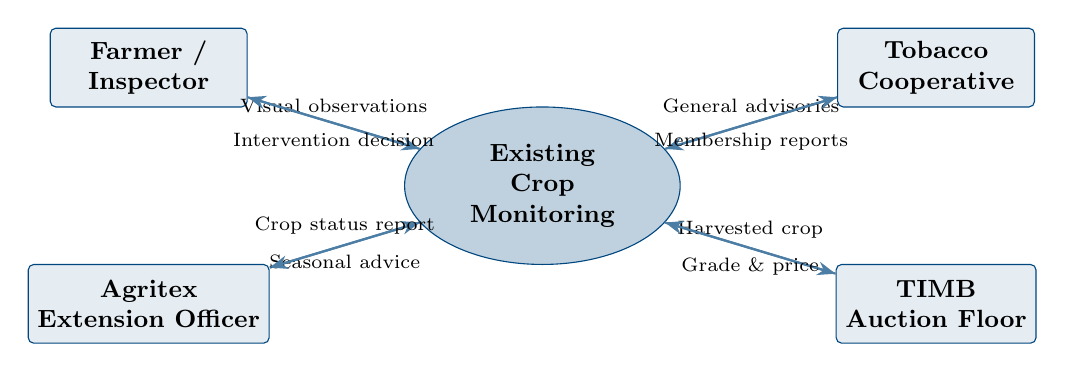
\begin{tikzpicture}[
  entity/.style={draw=hitblue,fill=hitblue!10,rectangle,minimum width=2.5cm,minimum height=1cm,
                 align=center,font=\small\bfseries,rounded corners=2pt},
  system/.style={draw=hitblue,fill=hitblue!25,ellipse,minimum width=3.5cm,minimum height=2cm,
                 align=center,font=\small\bfseries},
  arr/.style={->,>=Stealth,thick,draw=hitblue!70}
]
  % Central system
  \node[system] (sys) at (0,0) {Existing\\Crop\\Monitoring};
  % External entities
  \node[entity] (farmer) at (-5, 1.5) {Farmer /\\Inspector};
  \node[entity] (agritex) at (-5,-1.5) {Agritex\\Extension Officer};
  \node[entity] (cooperative) at (5, 1.5) {Tobacco\\Cooperative};
  \node[entity] (timb) at (5,-1.5) {TIMB\\Auction Floor};
  % Flows
  \draw[arr] (farmer) -- node[above,font=\scriptsize]{Visual observations} (sys);
  \draw[arr] (sys) -- node[below,font=\scriptsize]{Intervention decision} (farmer);
  \draw[arr] (agritex) -- node[below,font=\scriptsize]{Seasonal advice} (sys);
  \draw[arr] (sys) -- node[above,font=\scriptsize]{Crop status report} (agritex);
  \draw[arr] (cooperative) -- node[above,font=\scriptsize]{General advisories} (sys);
  \draw[arr] (sys) -- node[below,font=\scriptsize]{Membership reports} (cooperative);
  \draw[arr] (sys) -- node[above,font=\scriptsize]{Harvested crop} (timb);
  \draw[arr] (timb) -- node[below,font=\scriptsize]{Grade \& price} (sys);
\end{tikzpicture}
\end{figure}

\subsection{Weaknesses of the Current System}

\begin{itemize}
  \item \textbf{Reactive detection:} Stress is identified only after visual symptoms develop, missing the pre-symptom window when intervention is most effective.
  \item \textbf{Incomplete spatial coverage:} Manual inspection covers only 5--15\% of field area per visit, leaving most of the field unmonitored.
  \item \textbf{No data continuity:} Absence of systematic record-keeping prevents trend analysis, making it impossible to detect slow-developing stress trajectories.
  \item \textbf{Subjectivity and variability:} Assessments depend on individual inspector experience and may vary significantly between observers or visits.
  \item \textbf{Weather data isolation:} Environmental conditions are not integrated with field observations, preventing correlation of stress events with precipitation and temperature anomalies.
  \item \textbf{High opportunity cost:} The labour and time required for regular manual field inspections represents a significant cost that limits monitoring frequency.
\end{itemize}

\section{Description of the Proposed Solution}

The Satellite-Based Tobacco Crop Health Monitoring System replaces and substantially extends the existing monitoring capability through the integration of five core components:

\begin{enumerate}
  \item \textbf{Interactive Field Definition:} Farmers define field boundaries by drawing polygons on a satellite basemap through the React-Leaflet web interface. Polygon coordinates are stored as GeoJSON in the PostgreSQL database.

  \item \textbf{Live Satellite NDVI Retrieval:} For each analysis request, the system submits the field polygon to the Google Earth Engine API, which retrieves all available cloud-free Sentinel-2 Level-2A imagery within a configurable 14-to-30-day window, computes per-pixel NDVI from Band 8 (NIR) and Band 4 (Red), and returns both aggregate statistics and the spatial NDVI distribution across the field.

  \item \textbf{Weather Data Integration:} Historical weather data for the analysis window is retrieved from the Open-Meteo API using the field centroid coordinates, providing daily temperature and precipitation records that are aggregated into the feature vector.

  \item \textbf{Machine Learning Classification:} A logistic regression classifier trained on ground-truth Sentinel-2 and weather observations classifies the field into one of three health states: \emph{Healthy}, \emph{Moderate Stress}, or \emph{High Stress}, based on five engineered features.

  \item \textbf{Explainable Recommendations:} A rule-based engine translates the classification and feature values into specific, evidence-linked farming recommendations, presented in plain language with the data observations that triggered each recommendation.
\end{enumerate}

\subsection{Context Diagram and Data Flow Diagrams}

Figure~\ref{fig:ctx_new} presents the context diagram for the proposed system, showing the information flows between the system and all external entities.

\begin{figure}[H]
\centering
\caption{Context Diagram — Proposed Satellite Crop Health Monitoring System}
\label{fig:ctx_new}
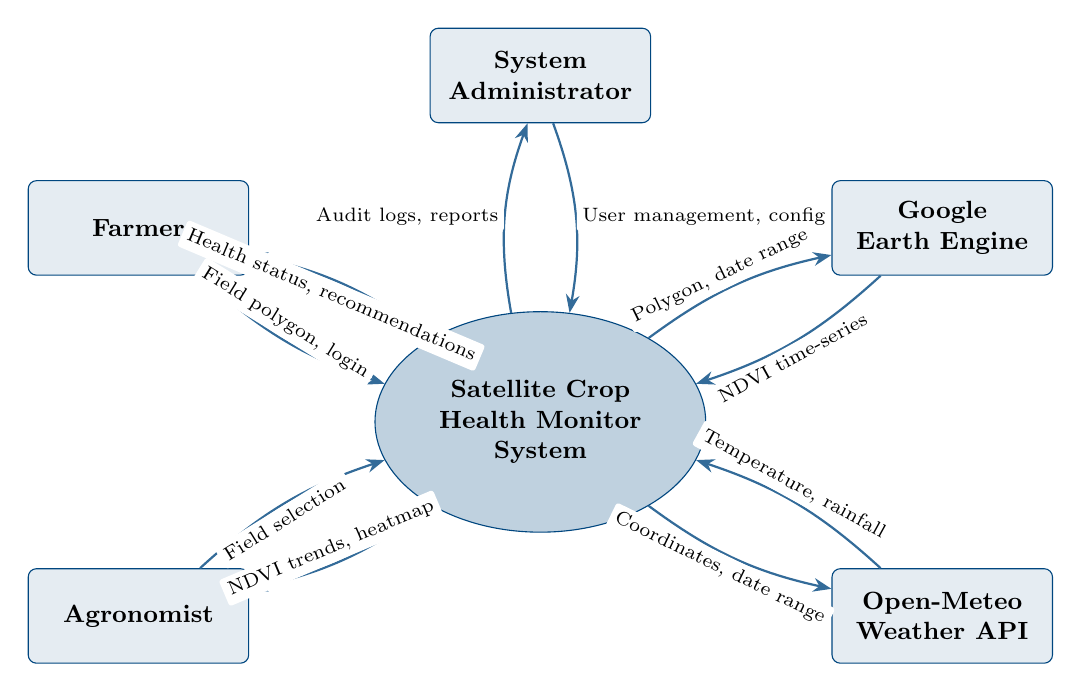
\begin{tikzpicture}[scale=0.88,
  entity/.style={draw=hitblue,fill=hitblue!10,rectangle,minimum width=2.8cm,minimum height=1.2cm,
                 align=center,font=\small\bfseries,rounded corners=3pt},
  system/.style={draw=hitblue,fill=hitblue!25,ellipse,minimum width=4.2cm,minimum height=2.8cm,
                 align=center,font=\small\bfseries},
  arr/.style={->,>=Stealth,thick,draw=hitblue!80},
  lbl/.style={font=\scriptsize,fill=white,inner sep=2pt,rounded corners=1pt}
]
  \node[system] (sys) at (0,0) {Satellite Crop\\Health Monitor\\System};

  % External entities — compass positions
  \node[entity] (farmer) at (-5.8,  2.8) {Farmer};
  \node[entity] (agro)   at (-5.8, -2.8) {Agronomist};
  \node[entity] (gee)    at ( 5.8,  2.8) {Google\\Earth Engine};
  \node[entity] (meteo)  at ( 5.8, -2.8) {Open-Meteo\\Weather API};
  \node[entity] (admin)  at ( 0,    5.0) {System\\Administrator};

  % Farmer <-> sys (bent to separate labels)
  \draw[arr] (farmer) to[bend right=12]
    node[lbl,above,sloped,pos=0.45]{Field polygon, login} (sys);
  \draw[arr] (sys) to[bend right=12]
    node[lbl,below,sloped,pos=0.55]{Health status, recommendations} (farmer);

  % Agronomist <-> sys
  \draw[arr] (agro) to[bend left=12]
    node[lbl,below,sloped,pos=0.45]{Field selection} (sys);
  \draw[arr] (sys) to[bend left=12]
    node[lbl,above,sloped,pos=0.55]{NDVI trends, heatmap} (agro);

  % GEE <-> sys
  \draw[arr] (sys) to[bend left=12]
    node[lbl,above,sloped,pos=0.45]{Polygon, date range} (gee);
  \draw[arr] (gee) to[bend left=12]
    node[lbl,below,sloped,pos=0.55]{NDVI time-series} (sys);

  % Open-Meteo <-> sys
  \draw[arr] (sys) to[bend right=12]
    node[lbl,below,sloped,pos=0.45]{Coordinates, date range} (meteo);
  \draw[arr] (meteo) to[bend right=12]
    node[lbl,above,sloped,pos=0.55]{Temperature, rainfall} (sys);

  % Admin <-> sys (vertical, straight with slight offset)
  \draw[arr] (admin) to[bend left=15]
    node[lbl,right]{User management, config} (sys);
  \draw[arr] (sys) to[bend left=15]
    node[lbl,left]{Audit logs, reports} (admin);
\end{tikzpicture}
\end{figure}

\noindent Figure~\ref{fig:dfd1} presents the Level 1 Data Flow Diagram, decomposing the system into its major processing components.

\begin{figure}[H]
\centering
\caption{Level 1 Data Flow Diagram — Proposed System}
\label{fig:dfd1}
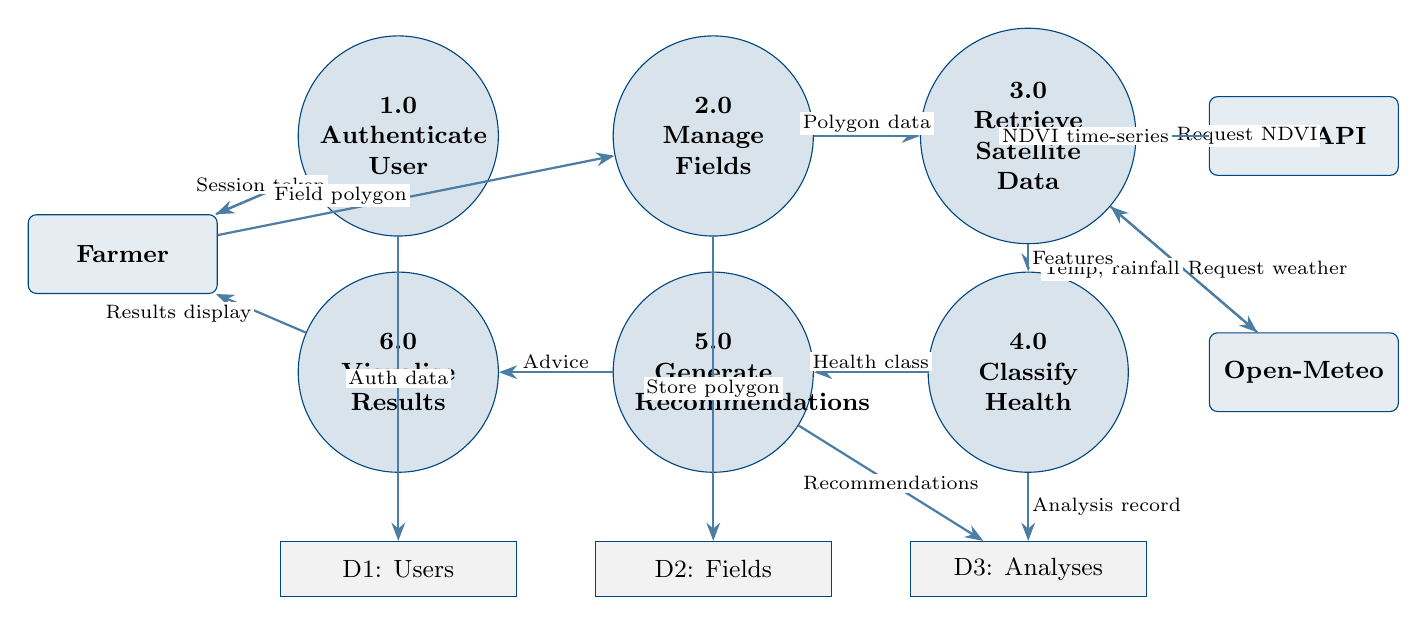
\begin{tikzpicture}[
  process/.style={draw=hitblue,circle,fill=hitblue!15,minimum size=2.2cm,
                  align=center,font=\small\bfseries,text width=2cm},
  store/.style={draw=hitblue,fill=gray!10,
                minimum width=3cm,minimum height=0.7cm,align=center,font=\small},
  ext/.style={draw=hitblue,fill=hitblue!10,rectangle,rounded corners=3pt,
              minimum width=2.4cm,minimum height=1cm,align=center,font=\small\bfseries},
  arr/.style={->,>=Stealth,draw=hitblue!70,thick},
  lbl/.style={font=\scriptsize,fill=white,inner sep=1pt}
]
  % Processes
  \node[process] (auth)  at (-4, 3)  {1.0\\Authenticate\\User};
  \node[process] (field) at (0,  3)  {2.0\\Manage\\Fields};
  \node[process] (sat)   at (4,  3)  {3.0\\Retrieve\\Satellite\\Data};
  \node[process] (ml)    at (4,  0)  {4.0\\Classify\\Health};
  \node[process] (rec)   at (0,  0)  {5.0\\Generate\\Recommendations};
  \node[process] (viz)   at (-4, 0)  {6.0\\Visualise\\Results};

  % Data stores
  \node[store] (users)    at (-4,-2.5) {D1: Users};
  \node[store] (fields)   at (0, -2.5) {D2: Fields};
  \node[store] (analyses) at (4, -2.5) {D3: Analyses};

  % External
  \node[ext] (farmer) at (-7.5, 1.5) {Farmer};
  \node[ext] (gee)    at (7.5,  3)   {GEE API};
  \node[ext] (meteo)  at (7.5,  0)   {Open-Meteo};

  % Flows
  \draw[arr] (farmer) -- node[lbl,above]{Credentials} (auth);
  \draw[arr] (auth) -- node[lbl,above]{Session token} (farmer);
  \draw[arr] (auth) -- node[lbl,above]{Auth data} (users);
  \draw[arr] (farmer) -- node[lbl,left,xshift=-2pt]{Field polygon} (field);
  \draw[arr] (field) -- node[lbl,above]{Polygon data} (sat);
  \draw[arr] (field) -- node[lbl]{Store polygon} (fields);
  \draw[arr] (sat) -- node[lbl,right]{Request NDVI} (gee);
  \draw[arr] (gee) -- node[lbl,left]{NDVI time-series} (sat);
  \draw[arr] (sat) -- node[lbl,right]{Request weather} (meteo);
  \draw[arr] (meteo) -- node[lbl,left]{Temp, rainfall} (sat);
  \draw[arr] (sat) -- node[lbl,right]{Features} (ml);
  \draw[arr] (ml) -- node[lbl,above]{Health class} (rec);
  \draw[arr] (rec) -- node[lbl,above]{Advice} (viz);
  \draw[arr] (viz) -- node[lbl,left,xshift=-2pt]{Results display} (farmer);
  \draw[arr] (ml) -- node[lbl,right]{Analysis record} (analyses);
  \draw[arr] (rec) -- node[lbl]{Recommendations} (analyses);
\end{tikzpicture}
\end{figure}

\section{Requirements Analysis}

\subsection{Functional Requirements}

The system's functional requirements, derived from user requirements and validated through questionnaire analysis, are summarised in Table~\ref{tab:functional}.

\begin{longtable}{>{\bfseries}p{0.8cm} p{4cm} p{7cm}}
\caption{Functional Requirements}\label{tab:functional}\\
\toprule
FR & Requirement Name & Description \\
\midrule
\endfirsthead
\toprule
FR & Requirement Name & Description \\
\midrule
\endhead
\bottomrule
\endfoot
FR01 & User Registration & The system shall allow new users to register with name, email, and password, validated against format and uniqueness constraints. \\[4pt]
FR02 & User Authentication & The system shall authenticate users against stored bcrypt-hashed passwords and issue HTTP-only session cookies on success. \\[4pt]
FR03 & Field Creation & The system shall enable authenticated farmers to create a field record by drawing a polygon on an interactive map and providing a field name. \\[4pt]
FR04 & Field Listing & The system shall display all fields belonging to the authenticated user with their names, areas, and last analysis dates. \\[4pt]
FR05 & Analysis Trigger & The system shall allow farmers to trigger a crop health analysis for any of their fields with a single user action. \\[4pt]
FR06 & Satellite NDVI Retrieval & The system shall query the Google Earth Engine API with the field polygon and a 14-to-30-day date range to retrieve Sentinel-2 NDVI time-series data. \\[4pt]
FR07 & Weather Data Retrieval & The system shall query the Open-Meteo API with the field centroid coordinates to retrieve daily temperature and precipitation data for the analysis window. \\[4pt]
FR08 & Feature Engineering & The system shall compute mean NDVI, NDVI trend slope, NDVI spatial variance, average temperature, and total rainfall from the retrieved satellite and weather data. \\[4pt]
FR09 & Health Classification & The system shall apply the trained logistic regression model to the engineered features and classify the field's health status as HEALTHY, MODERATE\_STRESS, or HIGH\_STRESS. \\[4pt]
FR10 & Recommendation Generation & The system shall apply four rule-based recommendation rules to the feature values and health classification to generate specific, evidence-linked farming advice. \\[4pt]
FR11 & Heatmap Visualisation & The system shall render a within-field NDVI heatmap overlay on the field map, highlighting spatial stress hotspots using a colour gradient. \\[4pt]
FR12 & Analysis History & The system shall store all analysis results and allow users to retrieve a history of analyses for each field. \\[4pt]
FR13 & Admin User Management & The system shall allow administrators to view, create, update, and deactivate user accounts. \\[4pt]
\end{longtable}

Figure~\ref{fig:usecase} presents the Use Case Diagram illustrating actor interactions with the system.

\begin{figure}[H]
\centering
\caption{Use Case Diagram — Satellite Crop Health Monitoring System}
\label{fig:usecase}
\resizebox{\linewidth}{!}{%
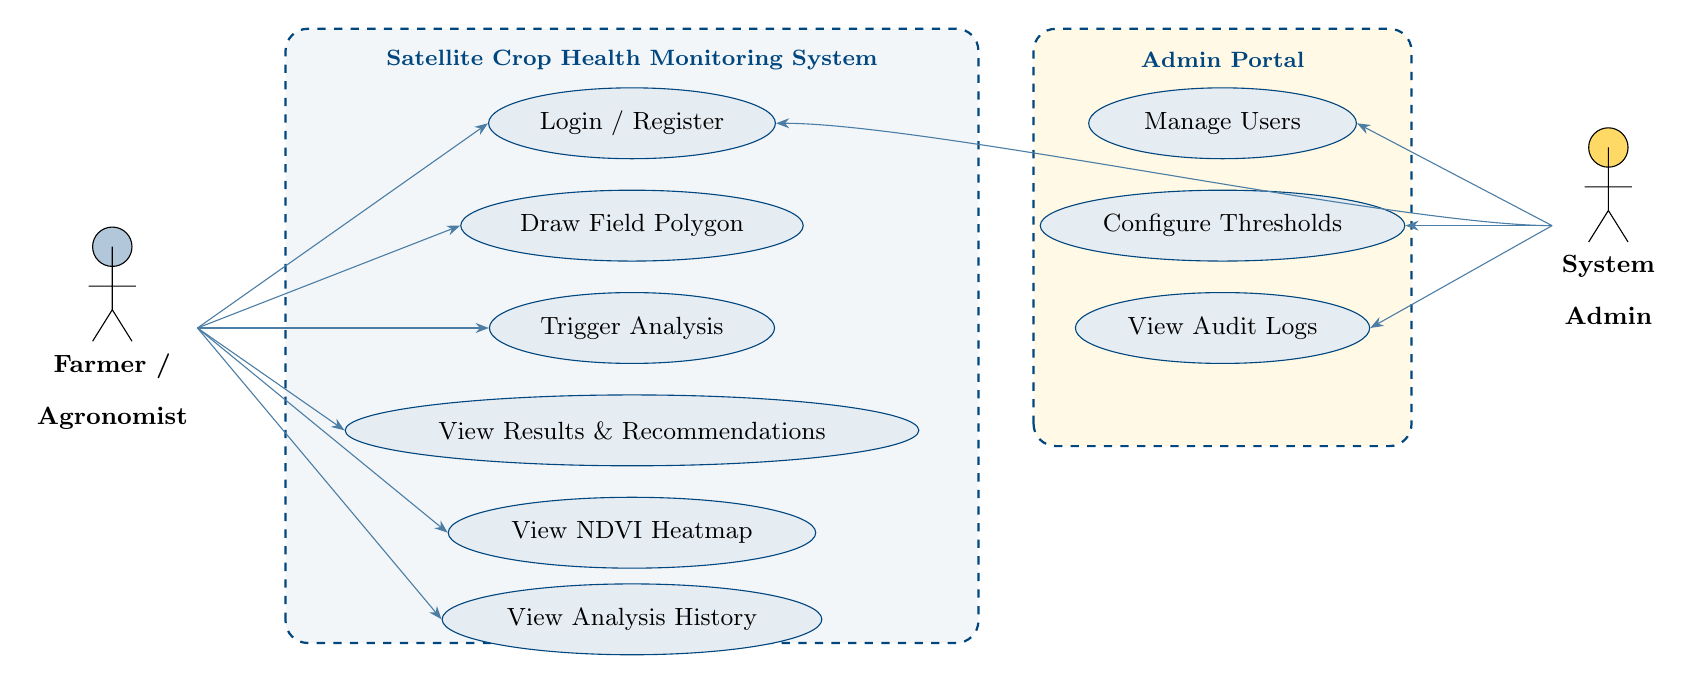
\begin{tikzpicture}[
  actor/.style={minimum width=1.2cm, minimum height=2cm, align=center, font=\small\bfseries},
  uc/.style={draw=hitblue,ellipse,fill=hitblue!10,minimum width=3.4cm, minimum height=0.9cm,
             align=center,font=\small},
  boundary/.style={draw=hitblue,thick,dashed,rounded corners=8pt},
  arr/.style={->,>=Stealth,draw=hitblue!70}
]
  % System boundary
  \draw[boundary,fill=hitblue!5] (-0.3,-6.3) rectangle (8.5, 1.5);
  \node[font=\footnotesize\bfseries,text=hitblue] at (4.1, 1.1) {Satellite Crop Health Monitoring System};

  % Use cases (inside boundary)
  \node[uc] (login)    at (4.1,  0.3) {Login / Register};
  \node[uc] (draw)     at (4.1, -1.0) {Draw Field Polygon};
  \node[uc] (analyse)  at (4.1, -2.3) {Trigger Analysis};
  \node[uc] (results)  at (4.1, -3.6) {View Results \& Recommendations};
  \node[uc] (heatmap)  at (4.1, -4.9) {View NDVI Heatmap};
  \node[uc] (history)  at (4.1, -6.0) {View Analysis History};

  % Admin use cases (separate section)
  \draw[boundary,fill=amber!10] (9.2,-3.8) rectangle (14.0, 1.5);
  \node[font=\footnotesize\bfseries,text=hitblue] at (11.6, 1.1) {Admin Portal};
  \node[uc] (manageusers) at (11.6, 0.3)  {Manage Users};
  \node[uc] (config)      at (11.6,-1.0)  {Configure Thresholds};
  \node[uc] (logs)        at (11.6,-2.3)  {View Audit Logs};

  % Actors
  \node[actor] (farmer) at (-2.5,-2.3)  {\tikz\draw[fill=hitblue!30](0,0.5)circle(0.25) (0,0.5)--(0,-0.3) (-0.3,0.0)--(0.3,0.0) (0,-0.3)--(-0.25,-0.7) (0,-0.3)--(0.25,-0.7);\\\vspace{0.2cm}Farmer /\\Agronomist};
  \node[actor] (admin)  at (16.5,-1.0)  {\tikz\draw[fill=amber!60](0,0.5)circle(0.25) (0,0.5)--(0,-0.3) (-0.3,0.0)--(0.3,0.0) (0,-0.3)--(-0.25,-0.7) (0,-0.3)--(0.25,-0.7);\\\vspace{0.2cm}System\\Admin};

  % Farmer connections
  \foreach \uc in {login,draw,analyse,results,heatmap,history}
    \draw[arr] (farmer.east) -- (\uc.west);

  % Admin connections
  \foreach \uc in {manageusers,config,logs}
    \draw[arr] (admin.west) -- (\uc.east);
  \draw[arr] (admin.west) to[out=180,in=0,looseness=0.5] (login.east);
\end{tikzpicture}%
}
\end{figure}

\subsection{Non-Functional Requirements}

\begin{itemize}
  \item \textbf{Performance:} The system shall complete a full crop health analysis—including satellite data retrieval, feature engineering, ML inference, and recommendation generation—within 30 seconds under normal network conditions. The web interface shall load within 3 seconds on a standard mobile data connection.

  \item \textbf{Security:} All user passwords shall be hashed using bcrypt with a minimum work factor of 12 before storage. Session management shall use HTTP-only cookies to prevent JavaScript-based session hijacking. The database shall enforce row-level access controls ensuring users can only access their own field and analysis records.

  \item \textbf{Reliability:} The system shall maintain availability during Zimbabwe's primary tobacco growing season (October to May). Analysis results shall be persisted in the database immediately upon completion to prevent data loss from connectivity interruptions. The system shall handle GEE or Open-Meteo API unavailability gracefully with appropriate user notification.

  \item \textbf{Usability:} The user interface shall be operable by a user with secondary school education and basic smartphone literacy, without requiring a user manual. Key actions—drawing a field and triggering analysis—shall be completable within five minutes by a first-time user. Health status shall be presented using colour-coded indicators (green, amber, red) that are interpretable without reading the accompanying text.

  \item \textbf{Scalability:} The database schema shall support an unlimited number of field records per user and shall use PostgreSQL with PostGIS to efficiently handle spatial queries as the system scales beyond 1,000 farmer records. The ML inference layer shall operate in JavaScript without requiring Python server infrastructure, enabling deployment to serverless platforms.

  \item \textbf{Compatibility:} The system shall function correctly on the latest two major versions of Chrome, Firefox, Safari, and Microsoft Edge on both desktop and mobile devices. The system shall be accessible on Android and iOS smartphones.

  \item \textbf{Maintainability:} The machine learning model shall be stored as a JSON weight file, enabling model updates to be deployed by file replacement without code changes. The recommendation rule configuration shall be stored in a separate threshold JSON file to enable agronomic threshold adjustments without redeployment.
\end{itemize}

\section{System Models}

\subsection{UML Activity Diagram}

Figure~\ref{fig:activity} presents the UML Activity Diagram for the primary crop health analysis workflow.

\begin{figure}[H]
\centering
\caption{UML Activity Diagram — Crop Health Analysis Workflow}
\label{fig:activity}
\resizebox{0.92\linewidth}{!}{%
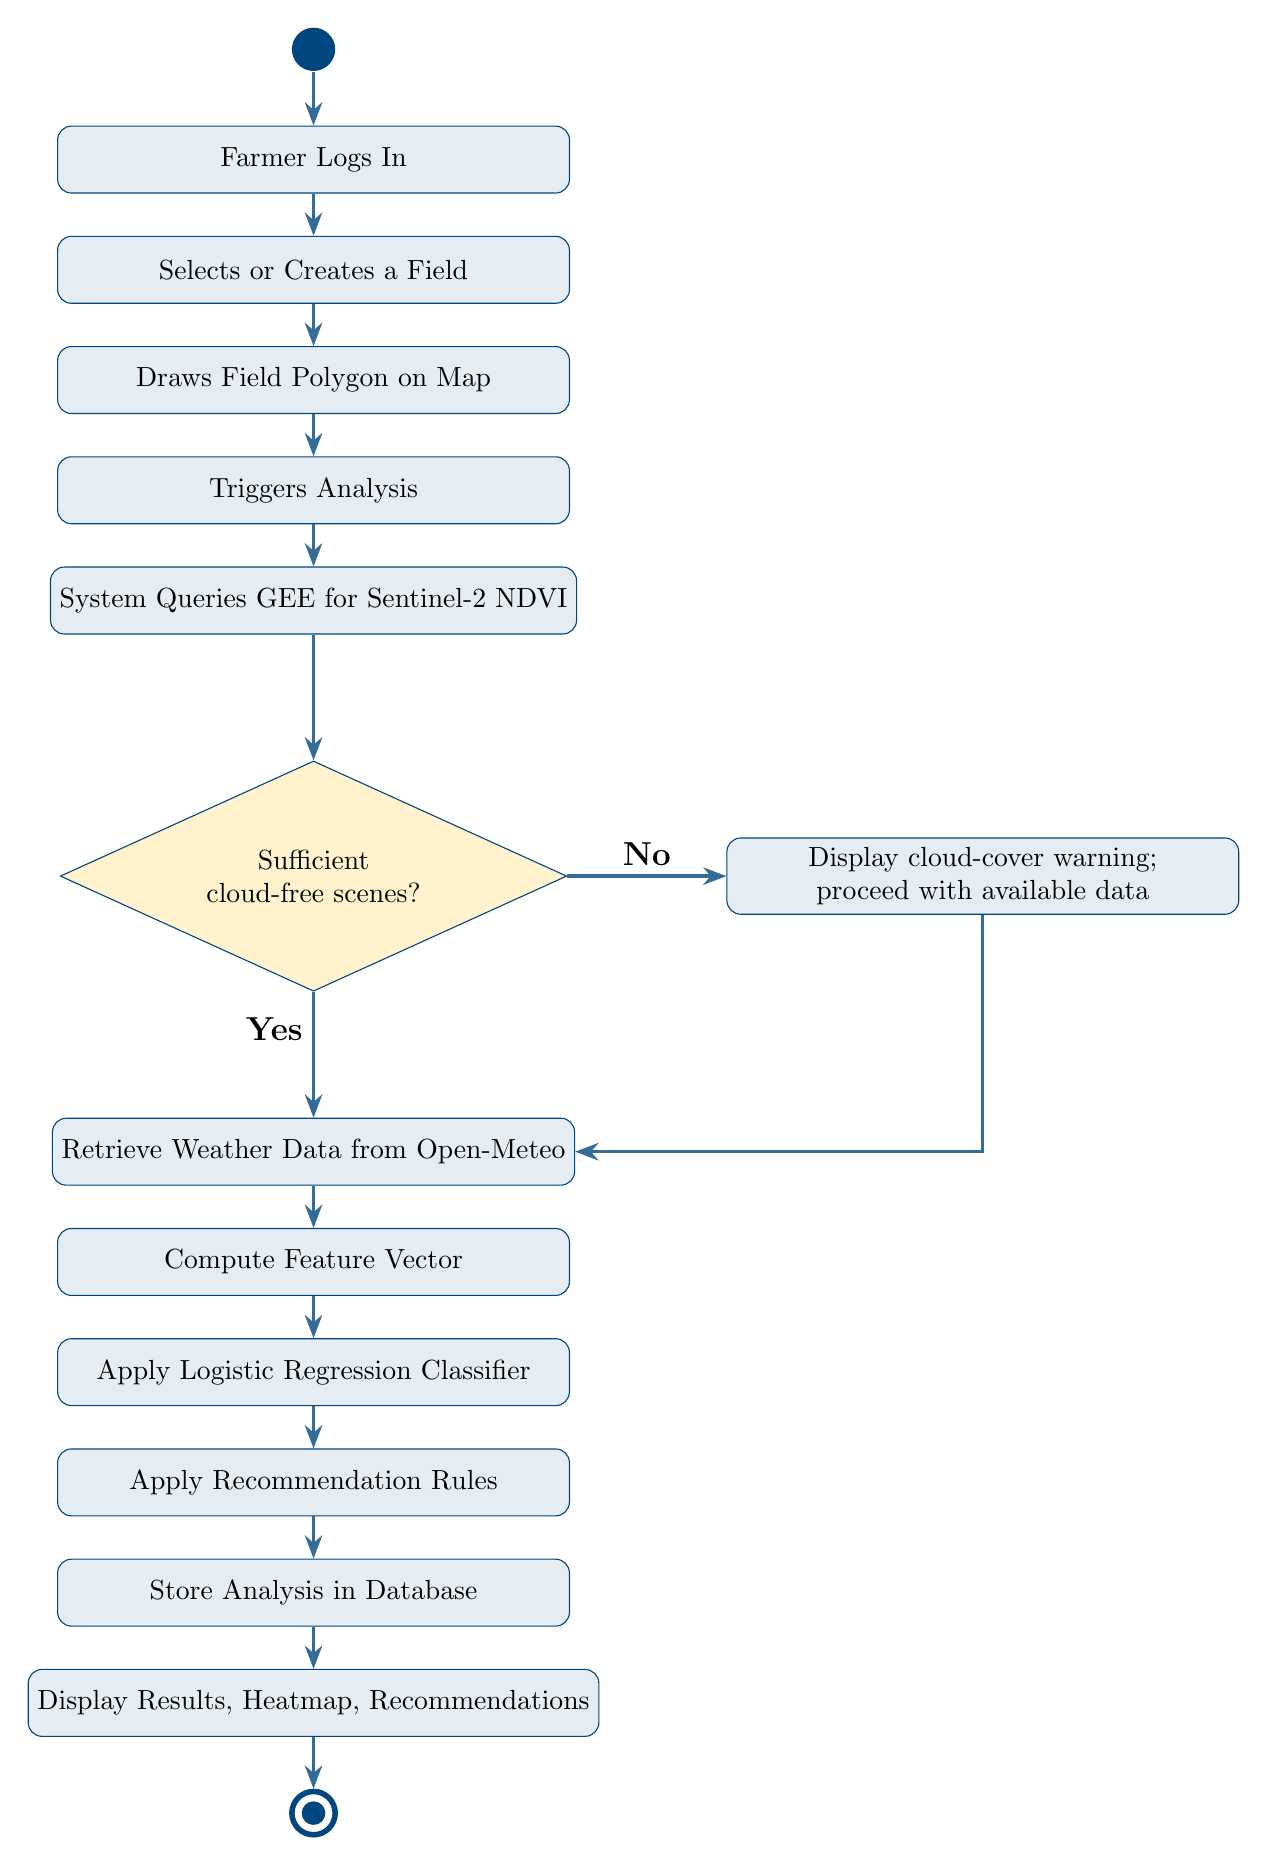
\begin{tikzpicture}[
  % Simple rounded-rectangle activities
  act/.style={draw=hitblue,fill=hitblue!10,rectangle,rounded corners=5pt,
              minimum width=6.5cm,minimum height=0.85cm,
              align=center,font=\normalsize},
  % Diamond — aspect=2.2 keeps it wide enough without being excessive
  dec/.style={draw=hitblue,fill=amber!20,diamond,aspect=2.2,
              inner sep=10pt,align=center,font=\normalsize},
  % Filled circle (start)
  start/.style={fill=hitblue,circle,minimum size=0.55cm},
  % Ring with filled inner circle (end)
  stop/.style={draw=hitblue,circle,minimum size=0.55cm,line width=2pt,
               path picture={\fill[hitblue](path picture bounding box.center)
                              circle (0.15cm);}},
  arr/.style={->,>=Stealth,draw=hitblue!80,line width=1.2pt}
]
  % ---- Nodes (1 unit = 1cm vertical step) ----
  \node[start]  (s)      at (0,  0)    {};
  \node[act]    (login)  at (0, -1.4)  {Farmer Logs In};
  \node[act]    (select) at (0, -2.8)  {Selects or Creates a Field};
  \node[act]    (draw)   at (0, -4.2)  {Draws Field Polygon on Map};
  \node[act]    (trig)   at (0, -5.6)  {Triggers Analysis};
  \node[act]    (gee)    at (0, -7.0)  {System Queries GEE for Sentinel-2 NDVI};
  % Decision diamond — extra vertical gap for readability
  \node[dec]    (cloud)  at (0,-10.5)  {Sufficient\\cloud-free scenes?};
  % "No" branch — same y as diamond
  \node[act]    (warn)   at (8.5,-10.5) {Display cloud-cover warning;\\proceed with available data};
  \node[act]    (wx)     at (0,-14.0)  {Retrieve Weather Data from Open-Meteo};
  \node[act]    (feat)   at (0,-15.4)  {Compute Feature Vector};
  \node[act]    (ml)     at (0,-16.8)  {Apply Logistic Regression Classifier};
  \node[act]    (rules)  at (0,-18.2)  {Apply Recommendation Rules};
  \node[act]    (store)  at (0,-19.6)  {Store Analysis in Database};
  \node[act]    (disp)   at (0,-21.0)  {Display Results, Heatmap, Recommendations};
  \node[stop]   (e)      at (0,-22.4)  {};

  % ---- Main flow ----
  \draw[arr] (s)      -- (login);
  \draw[arr] (login)  -- (select);
  \draw[arr] (select) -- (draw);
  \draw[arr] (draw)   -- (trig);
  \draw[arr] (trig)   -- (gee);
  \draw[arr] (gee)    -- (cloud);

  % ---- Decision branches ----
  % "Yes" — straight down from diamond south
  \draw[arr] (cloud.south) -- node[left,font=\large\bfseries,pos=0.3]{Yes} (wx.north);
  % "No"  — right from diamond east, then down-and-left back to main flow
  \draw[arr] (cloud.east)  -- node[above,font=\large\bfseries]{No} (warn.west);
  \draw[arr] (warn.south)  |- (wx.east);

  % ---- Rest of main flow ----
  \draw[arr] (wx)    -- (feat);
  \draw[arr] (feat)  -- (ml);
  \draw[arr] (ml)    -- (rules);
  \draw[arr] (rules) -- (store);
  \draw[arr] (store) -- (disp);
  \draw[arr] (disp)  -- (e);
\end{tikzpicture}%
}
\end{figure}

\subsection{UML Class Diagram}

Figure~\ref{fig:class} presents the UML Class Diagram for the system's data model as defined in the Prisma schema.

\begin{figure}[H]
\centering
\caption{UML Class Diagram — System Data Model}
\label{fig:class}
\resizebox{\linewidth}{!}{%
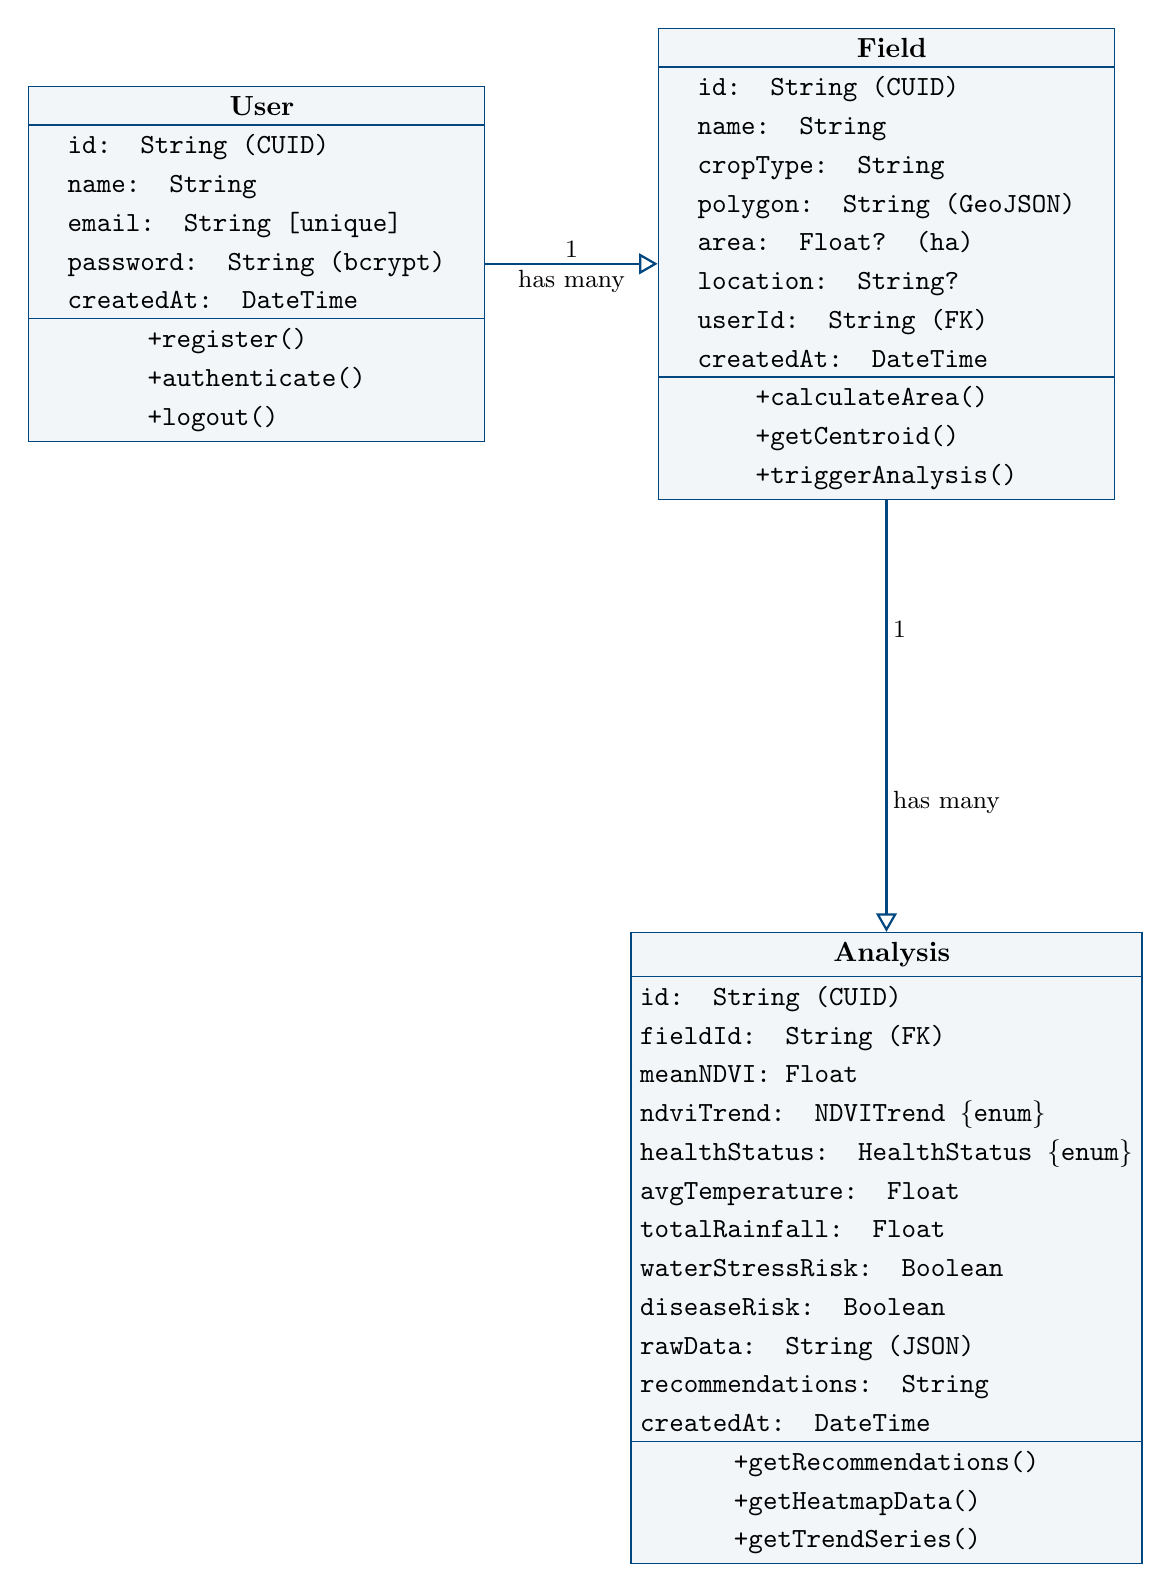
\begin{tikzpicture}[
  class/.style={draw=hitblue,fill=hitblue!5,rectangle split,rectangle split parts=3,
                minimum width=5.8cm,font=\normalsize,align=left,
                rectangle split part fill={hitblue!25,hitblue!5,hitblue!5}},
  link/.style={draw=hitblue,thick,>=open triangle 60},
  lbl/.style={font=\small,fill=white,inner sep=2pt}
]
  %% ---- User (left column, centred vertically on Field) ----
  \node[class] (user) at (0,0) {
    \textbf{\ User}
    \nodepart{two}
    \texttt{id: String (CUID)} \\[2pt]
    \texttt{name: String} \\[2pt]
    \texttt{email: String [unique]} \\[2pt]
    \texttt{password: String (bcrypt)} \\[2pt]
    \texttt{createdAt: DateTime}
    \nodepart{three}
    \texttt{+register()} \\[2pt]
    \texttt{+authenticate()} \\[2pt]
    \texttt{+logout()}
  };

  %% ---- Field (right column, same baseline as User) ----
  \node[class] (field) at (8,0) {
    \textbf{\ Field}
    \nodepart{two}
    \texttt{id: String (CUID)} \\[2pt]
    \texttt{name: String} \\[2pt]
    \texttt{cropType: String} \\[2pt]
    \texttt{polygon: String (GeoJSON)} \\[2pt]
    \texttt{area: Float? (ha)} \\[2pt]
    \texttt{location: String?} \\[2pt]
    \texttt{userId: String (FK)} \\[2pt]
    \texttt{createdAt: DateTime}
    \nodepart{three}
    \texttt{+calculateArea()} \\[2pt]
    \texttt{+getCentroid()} \\[2pt]
    \texttt{+triggerAnalysis()}
  };

  %% ---- Analysis (below Field — far enough to clear Field.south) ----
  \node[class] (analysis) at (8,-12.5) {
    \textbf{\ Analysis}
    \nodepart{two}
    \texttt{id: String (CUID)} \\[2pt]
    \texttt{fieldId: String (FK)} \\[2pt]
    \texttt{meanNDVI: Float} \\[2pt]
    \texttt{ndviTrend: NDVITrend \{enum\}} \\[2pt]
    \texttt{healthStatus: HealthStatus \{enum\}} \\[2pt]
    \texttt{avgTemperature: Float} \\[2pt]
    \texttt{totalRainfall: Float} \\[2pt]
    \texttt{waterStressRisk: Boolean} \\[2pt]
    \texttt{diseaseRisk: Boolean} \\[2pt]
    \texttt{rawData: String (JSON)} \\[2pt]
    \texttt{recommendations: String} \\[2pt]
    \texttt{createdAt: DateTime}
    \nodepart{three}
    \texttt{+getRecommendations()} \\[2pt]
    \texttt{+getHeatmapData()} \\[2pt]
    \texttt{+getTrendSeries()}
  };

  %% ---- Relationships ----
  % User 1 --< Field
  \draw[->,link] (user.east) -- node[lbl,above]{1}
                                node[lbl,below]{has many}
                                (field.west);

  % Field 1 --< Analysis (vertical)
  \draw[->,link] (field.south) -- node[lbl,right,pos=0.3]{1}
                                  node[lbl,right,pos=0.7]{has many}
                                  (analysis.north);
\end{tikzpicture}%
}
\end{figure}

\subsection{UML Sequence Diagram}

Figure~\ref{fig:sequence} presents the UML Sequence Diagram for the crop health analysis interaction, showing message flows between system components.

\begin{figure}[H]
\centering
\caption{UML Sequence Diagram — Crop Health Analysis Request}
\label{fig:sequence}
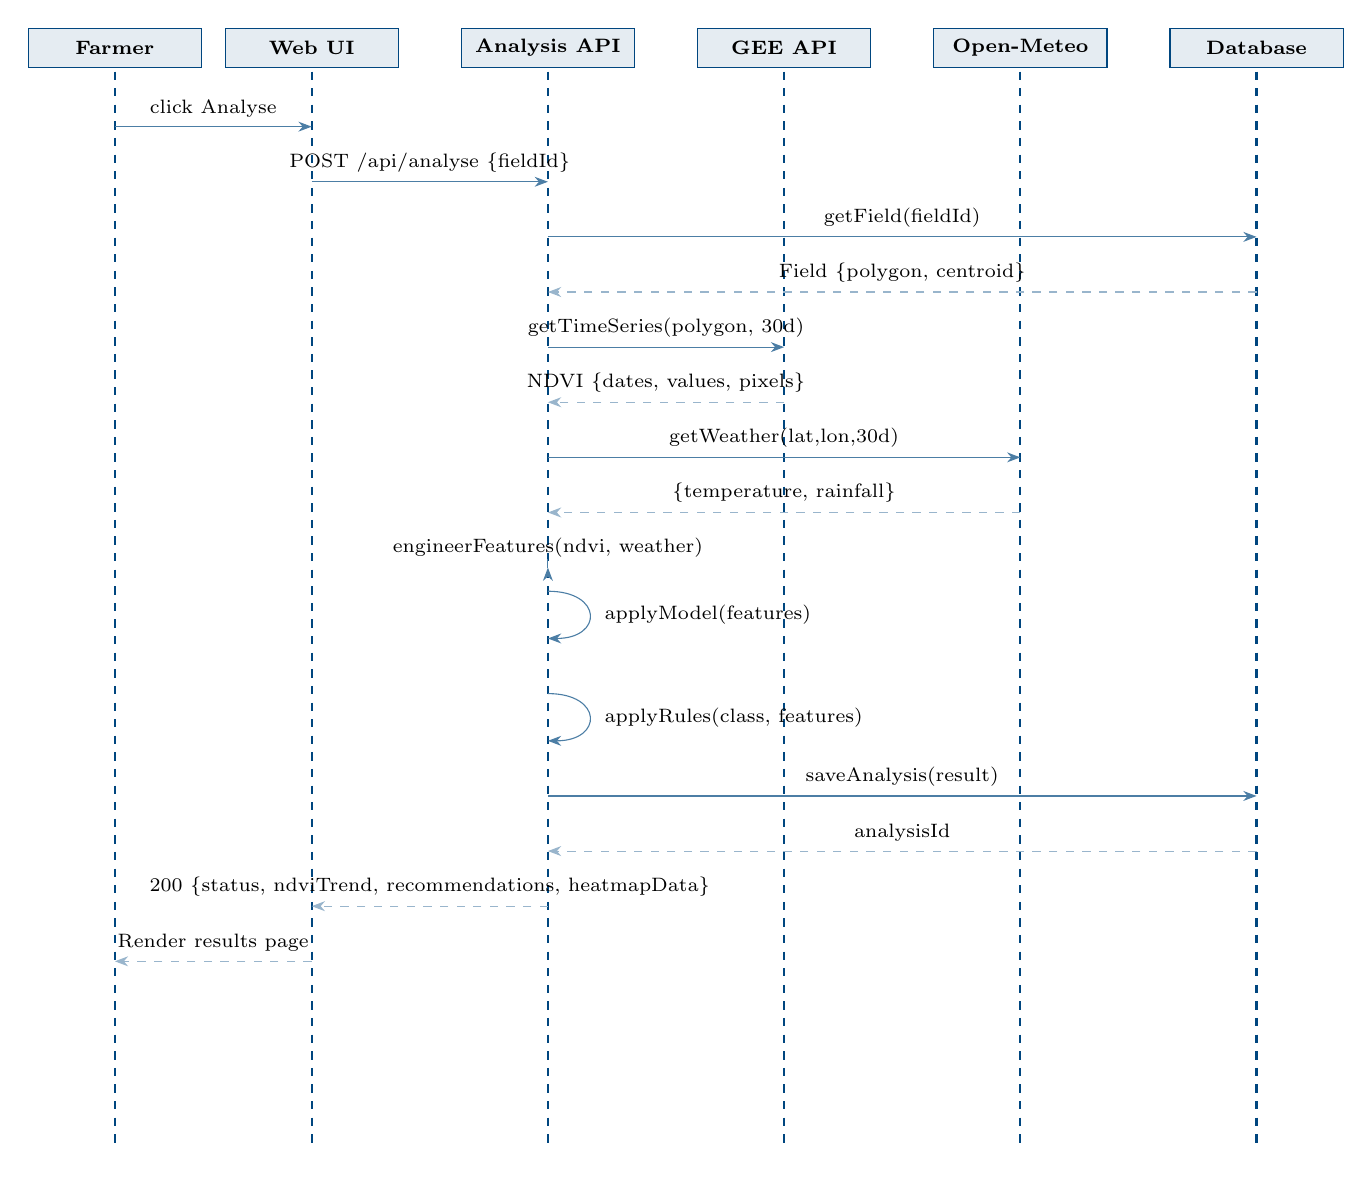
\begin{tikzpicture}[
  lifeline/.style={draw=hitblue,thick},
  msg/.style={->,>=Stealth,draw=hitblue!70,font=\scriptsize},
  ret/.style={->,>=Stealth,draw=hitblue!40,dashed,font=\scriptsize},
  box/.style={draw=hitblue,fill=hitblue!10,rectangle,minimum width=2.2cm,
              minimum height=0.5cm,align=center,font=\scriptsize\bfseries}
]
  % Lifeline headers
  \foreach \x/\lbl in {0/Farmer, 2.5/Web UI, 5.5/Analysis API, 8.5/GEE API, 11.5/Open-Meteo, 14.5/Database} {
    \node[box] at (\x*1cm,0) {\lbl};
    \draw[lifeline,dashed] (\x*1cm,-0.3) -- (\x*1cm,-14);
  }

  % Messages
  \def\yy{-1.0}
  \draw[msg] (0,-1.0) -- node[above]{\scriptsize click Analyse} (2.5,-1.0);
  \draw[msg] (2.5,-1.7) -- node[above]{\scriptsize POST /api/analyse \{fieldId\}} (5.5,-1.7);
  \draw[msg] (5.5,-2.4) -- node[above]{\scriptsize getField(fieldId)} (14.5,-2.4);
  \draw[ret] (14.5,-3.1) -- node[above]{\scriptsize Field \{polygon, centroid\}} (5.5,-3.1);
  \draw[msg] (5.5,-3.8) -- node[above]{\scriptsize getTimeSeries(polygon, 30d)} (8.5,-3.8);
  \draw[ret] (8.5,-4.5) -- node[above]{\scriptsize NDVI \{dates, values, pixels\}} (5.5,-4.5);
  \draw[msg] (5.5,-5.2) -- node[above]{\scriptsize getWeather(lat,lon,30d)} (11.5,-5.2);
  \draw[ret] (11.5,-5.9) -- node[above]{\scriptsize \{temperature, rainfall\}} (5.5,-5.9);
  \draw[msg] (5.5,-6.6) -- node[above]{\scriptsize engineerFeatures(ndvi, weather)} (5.5,-6.6);
  % Self-call indication
  \draw[msg] (5.5,-6.9) to[out=0,in=0,looseness=3] node[right,xshift=2pt]{\scriptsize applyModel(features)} (5.5,-7.5);
  \draw[msg] (5.5,-8.2) to[out=0,in=0,looseness=3] node[right,xshift=2pt]{\scriptsize applyRules(class, features)} (5.5,-8.8);
  \draw[msg] (5.5,-9.5) -- node[above]{\scriptsize saveAnalysis(result)} (14.5,-9.5);
  \draw[ret] (14.5,-10.2) -- node[above]{\scriptsize analysisId} (5.5,-10.2);
  \draw[ret] (5.5,-10.9) -- node[above]{\scriptsize 200 \{status, ndviTrend, recommendations, heatmapData\}} (2.5,-10.9);
  \draw[ret] (2.5,-11.6) -- node[above]{\scriptsize Render results page} (0,-11.6);
\end{tikzpicture}
\end{figure}

\noindent The sequence diagram illustrates the full analysis pipeline from farmer interaction through to result rendering. The Analysis API orchestrates all data retrieval from the GEE and Open-Meteo APIs, performs feature engineering and ML inference internally, and persists the result to the database before returning the formatted response to the web client.

% ============================================================
%  REFERENCES
% ============================================================
\clearpage
\addcontentsline{toc}{chapter}{References}
\markboth{REFERENCES}{}

\begin{thebibliography}{99}

\bibitem[\protect\citeauthoryear{Bégué et al.}{Bégué et al.}{2018}]{begue2018}
Bégué, A., Arvor, D., Bellon, B., Betbeder, J., de Abelleyra, D., Ferraz, R.P.D., Lebourgeois, V., Lelong, C., Simões, M. and Verón, S.R. (2018) `Remote sensing and cropping practices: a review', \textit{Remote Sensing}, 10(1), p. 99.

\bibitem[\protect\citeauthoryear{Breiman}{Breiman}{2001}]{breiman2001}
Breiman, L. (2001) `Random forests', \textit{Machine Learning}, 45(1), pp. 5--32.

\bibitem[\protect\citeauthoryear{Chlingaryan, Sukkarieh and Whelan}{Chlingaryan et al.}{2018}]{chlingaryan2018}
Chlingaryan, A., Sukkarieh, S. and Whelan, B. (2018) `Machine learning approaches for crop yield prediction and nitrogen status estimation in precision agriculture: a review', \textit{Computers and Electronics in Agriculture}, 151, pp. 61--69.

\bibitem[\protect\citeauthoryear{Climate Corporation}{Climate Corporation}{2023}]{climcorp2023}
Climate Corporation (2023) \textit{Climate FieldView Platform Documentation}. Available at: https://climate.com/fieldview (Accessed: 5 February 2025).

\bibitem[\protect\citeauthoryear{CropIn Technology}{CropIn Technology}{2023}]{cropin2023}
CropIn Technology (2023) \textit{SmartFarm Platform Overview}. Available at: https://www.cropin.com (Accessed: 10 February 2025).

\bibitem[\protect\citeauthoryear{Digital Green}{Digital Green}{2023}]{digitalgreen2023}
Digital Green (2023) \textit{Digital Green Technology Platform}. Available at: https://www.digitalgreen.org (Accessed: 12 February 2025).

\bibitem[\protect\citeauthoryear{European Space Agency}{ESA}{2023}]{esa2023}
European Space Agency (2023) \textit{Sentinel-2 User Handbook}. 2nd edn. Paris: ESA.

\bibitem[\protect\citeauthoryear{Farmerline}{Farmerline}{2023}]{farmerline2023}
Farmerline (2023) \textit{Farmerline Smart Farming Tools}. Available at: https://farmerline.co (Accessed: 10 February 2025).

\bibitem[\protect\citeauthoryear{Food and Agriculture Organization of the United Nations}{FAO}{2023}]{fao2023}
Food and Agriculture Organization of the United Nations (2023) \textit{FAOSTAT: Crops and Livestock Products}. Available at: https://www.fao.org/faostat (Accessed: 10 January 2025).

\bibitem[\protect\citeauthoryear{Gebbers and Adamchuk}{Gebbers and Adamchuk}{2010}]{gebbers2010}
Gebbers, R. and Adamchuk, V.I. (2010) `Precision agriculture and food security', \textit{Science}, 327(5967), pp. 828--831.

\bibitem[\protect\citeauthoryear{Gorelick et al.}{Gorelick et al.}{2017}]{gorelick2017}
Gorelick, N., Hancher, M., Dixon, M., Ilyushchenko, S., Thau, D. and Moore, R. (2017) `Google Earth Engine: planetary-scale geospatial analysis for everyone', \textit{Remote Sensing of Environment}, 202, pp. 18--27.

\bibitem[\protect\citeauthoryear{Kamilaris and Prenafeta-Boldú}{Kamilaris and Prenafeta-Boldú}{2018}]{kamilaris2018}
Kamilaris, A. and Prenafeta-Boldú, F.X. (2018) `Deep learning in agriculture: a survey', \textit{Computers and Electronics in Agriculture}, 147, pp. 70--90.

\bibitem[\protect\citeauthoryear{Liakos et al.}{Liakos et al.}{2018}]{liakos2018}
Liakos, K.G., Busato, P., Moshou, D., Pearson, S. and Bochtis, D. (2018) `Machine learning in agriculture: a review', \textit{Sensors}, 18(8), p. 2674.

\bibitem[\protect\citeauthoryear{Ministry of Lands, Agriculture, Fisheries, Water and Rural Development}{Ministry of Agriculture}{2022}]{moa2022}
Ministry of Lands, Agriculture, Fisheries, Water and Rural Development (2022) \textit{Zimbabwe Agricultural Development Strategy II (2021--2025)}. Harare: Government of Zimbabwe.

\bibitem[\protect\citeauthoryear{Nyoka, Dube and Masocha}{Nyoka et al.}{2020}]{nyoka2020}
Nyoka, M., Dube, T. and Masocha, M. (2020) `Assessing the utility of remote sensing data in monitoring tobacco crop health in Zimbabwe', \textit{South African Geographical Journal}, 102(1), pp. 15--32.

\bibitem[\protect\citeauthoryear{Open-Meteo}{Open-Meteo}{2023}]{openmeteo2023}
Open-Meteo (2023) \textit{Open-Meteo Weather API Documentation}. Available at: https://open-meteo.com/en/docs (Accessed: 20 January 2025).

\bibitem[\protect\citeauthoryear{Pedregosa et al.}{Pedregosa et al.}{2011}]{pedregosa2011}
Pedregosa, F., Varoquaux, G., Gramfort, A., Michel, V., Thirion, B., Grisel, O., Blondel, M., Prettenhofer, P., Weiss, R., Dubourg, V. and Vanderplas, J. (2011) `Scikit-learn: machine learning in Python', \textit{Journal of Machine Learning Research}, 12, pp. 2825--2830.

\bibitem[\protect\citeauthoryear{Perera, Liu and Jayawardena}{Perera et al.}{2015}]{perera2015}
Perera, C., Liu, C.H. and Jayawardena, S. (2015) `The emerging Internet of Things marketplace from an industrial perspective: a survey', \textit{IEEE Transactions on Emerging Topics in Computing}, 3(4), pp. 585--598.

\bibitem[\protect\citeauthoryear{Pfleeger and Atlee}{Pfleeger and Atlee}{2010}]{pfleeger2010}
Pfleeger, S.L. and Atlee, J.M. (2010) \textit{Software Engineering: Theory and Practice}. 4th edn. Upper Saddle River, NJ: Pearson.

\bibitem[\protect\citeauthoryear{PostgreSQL Global Development Group}{PostgreSQL}{2023}]{postgresql2023}
PostgreSQL Global Development Group (2023) \textit{PostgreSQL 16 Documentation}. Available at: https://www.postgresql.org/docs/16 (Accessed: 15 January 2025).

\bibitem[\protect\citeauthoryear{Prisma}{Prisma}{2023}]{prisma2023}
Prisma (2023) \textit{Prisma ORM Documentation}. Available at: https://www.prisma.io/docs (Accessed: 15 January 2025).

\bibitem[\protect\citeauthoryear{Regrow Ag}{Regrow Ag}{2023}]{regrow2023}
Regrow Ag (2023) \textit{Regrow Sustainable Agriculture Platform}. Available at: https://www.regrow.ag (Accessed: 15 February 2025).

\bibitem[\protect\citeauthoryear{Rose et al.}{Rose et al.}{2016}]{rose2016}
Rose, D.C., Sutherland, W.J., Parker, C., Lobley, M., Winter, M., Morris, C., Twining, S., Ffoulkes, C., Amano, T. and Dicks, L.V. (2016) `Decision support tools for agriculture: towards effective design and delivery', \textit{Agricultural Systems}, 149, pp. 165--174.

\bibitem[\protect\citeauthoryear{Rouse et al.}{Rouse et al.}{1974}]{rouse1974}
Rouse, J.W., Haas, R.H., Schell, J.A. and Deering, D.W. (1974) `Monitoring vegetation systems in the Great Plains with ERTS', in \textit{Third Earth Resources Technology Satellite-1 Symposium}, vol. 1. Greenbelt, MD: NASA, pp. 309--317.

\bibitem[\protect\citeauthoryear{Rwizi, Sibanda and Chimonyo}{Rwizi et al.}{2021}]{rwizi2021}
Rwizi, T.L., Sibanda, M. and Chimonyo, V.G.P. (2021) `Use of satellite data for agricultural applications in Zimbabwe: opportunities and challenges', \textit{Zimbabwe Journal of Agricultural Sciences}, 3(1), pp. 22--38.

\bibitem[\protect\citeauthoryear{SatAgro}{SatAgro}{2023}]{satagtro2023}
SatAgro (2023) \textit{SatAgro Satellite Monitoring Service}. Available at: https://satagtro.com (Accessed: 12 February 2025).

\bibitem[\protect\citeauthoryear{Sommerville}{Sommerville}{2016}]{sommerville2016}
Sommerville, I. (2016) \textit{Software Engineering}. 10th edn. Harlow: Pearson Education.

\bibitem[\protect\citeauthoryear{Taranis}{Taranis}{2023}]{taranis2023}
Taranis (2023) \textit{Taranis Aerial Intelligence Platform}. Available at: https://taranis.ag (Accessed: 5 February 2025).

\bibitem[\protect\citeauthoryear{Tobacco Industry and Marketing Board}{TIMB}{2023}]{timb2023}
Tobacco Industry and Marketing Board (2023) \textit{Annual Report 2022/2023}. Harare: TIMB.

\bibitem[\protect\citeauthoryear{Tucker}{Tucker}{1979}]{tucker1979}
Tucker, C.J. (1979) `Red and photographic infrared linear combinations for monitoring vegetation', \textit{Remote Sensing of Environment}, 8(2), pp. 127--150.

\bibitem[\protect\citeauthoryear{Weiss, Jacob and Duveiller}{Weiss et al.}{2020}]{weiss2020}
Weiss, M., Jacob, F. and Duveiller, G. (2020) `Remote sensing for agricultural applications: a meta-review', \textit{Remote Sensing of Environment}, 236, p. 111402.

\bibitem[\protect\citeauthoryear{Wieringa}{Wieringa}{2014}]{wieringa2014}
Wieringa, R.J. (2014) \textit{Design Science Methodology for Information Systems and Software Engineering}. Berlin: Springer.

\bibitem[\protect\citeauthoryear{Wolfert et al.}{Wolfert et al.}{2017}]{wolfert2017}
Wolfert, S., Ge, L., Verdouw, C. and Bogaardt, M.J. (2017) `Big data in smart farming: a review', \textit{Agricultural Systems}, 153, pp. 69--80.

\end{thebibliography}

\end{document}
